\section{Overview}\label{sec:supervised:overview}

I will introduce in the present chapter the basis on which I will build the
work of the thesis. In the following chapters I will incrementally construct
over what is developed in this chapter. The results of this chapter will be
used as a baseline to assess the impact of the additions worked on subsequent
chapters.

Recapitulating on Chapter \ref{chapter:introduction}, Section
\ref{section:introduction:overview}, I state the problem at hand. I have
available a labeled dataset of disambiguated verb senses which is small.
Developing a manual annotated resource is expensive because the manual
annotation is done by domain experts. Because of the nature of language the
distribution of the classes (i.e. senses) in the dataset is Zipfian
\cite{j:zpf}. Therefore I have a resource where the distribution of the
annotations is highly biased toward a most frequent class. This resource poses
two challenges: the number of annotated examples, and the distribution of the
labels.

To obtain an algorithm for \vsd~the simplest approach is to train a supervised
automatic classifier. However with a purely supervised approach and as
consequence of the challenges stated above, I have to deal with two problems:
overfitting of the data and bias of the algorithm to tag everything as the most
frequent class. I will show these problems exist and discuss with the results
and conclusions of this chapter what I can do to improve the learning process
to overcome these problems.

To explore these challenges I formalize so with the following Hypothesis:

\begin{hypothesis}\label{hyp:supervised}
  The size of the dataset affects the quality of the final model.
\end{hypothesis}

In order to accept or reject such Hypothesis, I divide it in more specific
ones:

\begin{subhypothesis}\label{hyp:supervised:1}
  With larger training sets, the performance improves. 
\end{subhypothesis}

\begin{subhypothesis}\label{hyp:supervised:2}
  With larger datasets the classifier is less prone to overfitting. 
\end{subhypothesis}

\begin{subhypothesis}\label{hyp:supervised:3}
  The number of classes affects the tendency to overfit.
\end{subhypothesis}

\begin{subhypothesis}\label{hyp:supervised:4}
  Linear models have less tendency to overfit than non-linear models.
\end{subhypothesis}

These hypotheses will be accepted or rejected using the following layout:

\begin{itemize}
  \item Experiment \ref{exp:supervised:2} reports the performance of a model as
    the number of examples increases. The performance is measured by the macro
    and weighted average F1-score (Metric \ref{met:1}). Results
    shown in Section \ref{sec:supervised:hyp:1} serve to accept Hypothesis
    \ref{hyp:supervised:1}, that the performance improve with larger training
    sets.
  \item Experiment \ref{exp:supervised:3} reports the variance of different
    models trained over different subsets of the training data. This variance
    is measured by Metric \ref{met:3} which reflects the tendency of
    a model to overfit, with aid of the learning curve. From this experiment
    and metric, using different visualizations according to the task, I show
    that the classifier is less prone to overfitting with larger datasets
    (Hypothesis \ref{hyp:supervised:2}, in Section \ref{sec:supervised:hyp:2}),
    with less classes (Hypothesis \ref{hyp:supervised:3}, in Section
    \ref{sec:supervised:hyp:3}). I also show that linear models have less
    tendency to overfit (Hypothesis \ref{hyp:supervised:4}, in Section
    \ref{sec:supervised:hyp:4}).
\end{itemize}

In Section \ref{sec:supervised:previous} I recapitulate on previous work done
in supervised learning for \wsd~both for English and Spanish, with a special
focus on \vsd~and the problem of learning with very few examples and class
imbalance.

In Section \ref{sec:supervised:methodology} I explain all relevant items
concerning what is used to carry out the experimentation of this chapter.
First, in Section \ref{sec:supervised:resources} I introduce the resources I
work with. The SenSem annotated corpus on which the rest of the Thesis's work
is done and SemEval Corpus for the sake of comparison with the standard and to
ensure that there is no language related bias. These resources are represented
in this stage with what I name {\em hand-crafted features} taken from the
resources themselves, this is what I present in Section
\ref{sec:supervised:features}. I also explore techniques to reduce the
dimensionality of the representations and see how this is a necessary step to
be able to train some classifiers. I introduce the classification algorithms
used for the automatic \wsd~task in Section \ref{sec:supervised:classifiers}.
Section \ref{sec:supervised:experiments} lists the experiments done. And
Section \ref{sec:supervised:metrics} lists the set of metrics I use to measure
the experiments.

Section \ref{sec:supervised:results} reports the results of the experiments and
analyses them in order to accept or reject the stated hypotheses of the
chapter.

Finally Section \ref{sec:supervised:conclusions} draws the conclusions of this
chapter, recapitulating the Hypotheses and accepting or rejecting them
according to the evidence gathered in the results. It states the shortcomings
of the methods explores in this chapter and what I want to accomplish on the
next and ends by listing the future work.

\section{Relevant Work}\label{sec:supervised:previous}

I recall from Chapter \ref{chapter:domain_background}, in Section
\ref{sec:domain_background:supervised}, there is some work done for English
\vsd~and some for Spanish~\wsd, but not much for Spanish \vsd. To my knowledge
the work done exclusively for Spanish \vsd~is almost non-existent. Moreover the
features used in English \vsd, like selectional preferences and abstract
semantic features, are not available for Spanish.

In particular, to design the supervised machine learning system I took
inspiration from the {\em It Make Sense} system
\cite{Zhong:2010:MSW:1858933.1858947}, and use a pipeline similar to theirs.

First, there was a preprocessing step of the labeled corpora where it was
analyzed automatically. Then I use the available information to generate
features to represent the instances to use as training data. Finally
different supervised classifiers were tried in the experimentation phase.

To design the features I was based on the work already mentioned in Section
\ref{sec:domain_background:supervised}. Specially from Ye and Baldwin
\cite{Ye:2006:ALTA2006}, M\`arquez et al. \cite{marquez07a}, and Montoyo et al.
\cite{DBLP:journals/corr/abs-1109-2130}.

\section{Methodology}\label{sec:supervised:methodology}

In this Section, I explain the general methods used to carry out the
experiments of this chapter. Once again, for the scope of this thesis, the
words {\em dataset} and {\em corpus} are interchangeable. On the other hand
when I use the word {\bf model} I mean the result of training a {\em
classifier} with a specific {\em representation} for a specific {\em corpus}.
 
\subsection{Resources}\label{sec:supervised:resources}

As the project focus mainly on \vsd, there are two corpora I worked with:
SenSem \cite{alonso-etal-07-sensem} labeled corpus of Spanish verb senses and
SemEval-2007 Task 17 \cite{Pradhan:2007:STE:1621474.1621490} corpus for
English.

The main focus is the work on SenSem as the areas of \wsd, in general, and
\vsd, in particular, for Spanish language can greatly benefit from the results
I can find; specially since the basic resource exists but is small and in
need of improvements. Plus, as this is the work from an Spanish born speaker,
it surely is a research interest of me.

SemEval, being of English language, is mostly used as a comparison to the work
for Spanish in this chapter, since the work in English in the area is more
solid than that of Spanish.

\subsubsection{SenSem}\label{sec:supervised:sensem}

SenSem \cite{alonso-etal-07-sensem} is a manually annotated corpus for both
Spanish and Catalan. It serves as main resource for the experiments in Spanish.
It contains the 248 most common verbs of Spanish, annotated with senses defined
in a provided lexicon, some of them with mappings to the Spanish Wordnet
Ontology \cite{DBLP:conf/konvens/MontravetaVF08}.

A version of the SenSem corpus has part-of-speech tags automatically annotated
with Freeling \cite{padro12}. However these tags are annotated on a word based
level, thus there is a large proportion of them annotated with the wrong tag
(e.g. verbs annotated as nouns). Furthermore, Spanish has some words that are
multi-words (i.e. words formed of two ore more different terms) which tag is
not the same than those of each of the words compounding the multi-word. E.g.
``m\'as\_all\'a\_de'' is tagged as a multi-word with Part-of-Speech tag ``SP'',
it is a preposition, however, the words ``m\'as'' and ``all\'a'' are by
themselves adverbs and only ``de'' is a preposition.

In order to gather information more useful for feature extraction, there was a
two step preprocessing of the SenSem corpus. First, an automatic annotation
using an statistical parser. In this step the SenSem's sentences, which are
tokenized, are given to Freeling. Using the statistical dependency parser, the
sentences are annotated with: lemma, part-of-speech tag, morphosyntactic
information and dependency triples. Also, there is multi-word detection and
named entity recognition (treated by Freeling as multi-words).

Nevertheless, the automatic annotation is not enough as errors come not only
from Freeling but other problem SenSem has as well: sentences without a defined
sense, sentences where the verb to disambiguate is not present and sentences
truncated before finishing. For this reason, the second step of preprocessing
was manual, where each of the automatically annotated sentences where the main
lemma to disambiguate was lost (because of mistagging, not being correctly
marked in the original resource, etc.), is found manually. Besides this, all
cases that are erroneous in the original corpus (e.g. truncated sentences or
sentences without a defined sense) were discarded. 

After the text preprocessing, the SenSem corpus was split in train/test. For
this all those senses with less than two occurrences in the corpus are filtered
out and the remaining senses are split with stratified sampling using 80\%
for training and 20\% for testing, where the train corpus has at least two
occurrences of every sense and the test corpus has at least one occurrence of
every sense. These splits also preserve the distribution of classes observed in
the whole dataset. This implies that in each split you cannot find more
examples of a class than you could find in a stratified sample of the dataset,
that is, a sample that preserves the distribution of the whole dataset.
However, this does not necessarily hold for minority classes, because at least
one example must be found in each split, even if that implies over-representing
the class.

The test corpus is always the same for every experiment in the thesis, and is
held out from training to use for measuring the performance of the different
algorithms studied in this thesis. I need two occurrences in the training
corpus of each sense because in the future experiments (the ones comprising
semi-supervised approach), a validation corpus is needed to aid the early
stopping criterion of the algorithms and thus the same approach for splitting
train and test corpus is used (in this case with at least one example per sense
for each split).

Table \ref{tab:sensem:stats} shows some of the statistics of the SenSem corpus
after the preprocessing of the text and removal of erroneous sentences. I want
to focus specially on the average number of instances for the most frequent
sense per lemma in comparison to the average number of instances for the second
most frequent sense per lemma. Is clear to see the imbalance of the senses in
the corpora as the most frequent class has more than 3 times more occurrences
than the next.

\begin{table}[ht]
  \centering
  \begin{tabular}{lr}
    \toprule
    \textbf{Statistic} & \textbf{Value} \\
    \midrule
    Total no. of instances (before filtering) & 23938 \\
    Total no. of instances (after filtering) & 20138 \\
    Total no. of lemmas (before filtering) & 248 \\
    Total no. of lemmas (after filtering) & 208 \\
    Total no. of senses (before filtering) & 772 \\
    Total no. of senses (after filtering) & 732 \\
    \midrule
    Average no. of senses per lemma & 3.52 \\
    Average no. of instances per lemma & 96.82 \\
    Average no. of instances per sense & 27.51 \\
    Average no. of instances for the most frequent sense per lemma & 67.08 \\
    Average no. of instances for the second most frequent sense per lemma & 19.67 \\
    \bottomrule
  \end{tabular}
  \caption{SenSem statistics}
  \label{tab:sensem:stats}
\end{table}

In summary, the original version of the SenSem was automatically parsed with
Freeling to gather more data to use for the features construction, and then was
manually revised in order to correct mistagging and discard incorrect sentences
(e.g. truncated sentences). After this, it was split in train and test
datasets.

\subsubsection{SemEval}

To compare the results with a standard experimental setting, I replicate
experiments using the SemEval-2007 Task-17 corpus
\cite{Pradhan:2007:STE:1621474.1621490}. The corpus has information of the
senses of 100 different lemmas, 65 verbs and 35 nouns (unlike SenSem which only
has information about verb senses). Since this work want to asses the results
of Spanish verb sense disambiguation, it was decided to leave out the 35 nouns
from the experimental settings of English and only work with the verbs.

Unlike SenSem, the SemEval corpus was already split in train and test
corpora. There are senses that only occur once in the whole corpus, either in
the train or in the test data. In order to not alter SemEval so is still useful
for comparison, no filtering of the dataset was done. However, given the
nature of the classifiers used here, those cases where the sense only exists in
the test corpus will have no way of being predicted by the classifiers.

Other differences between SenSem and SemEval is the way the examples are
presented. In SenSem each example represents only one sentence where a specific
token is the one being disambiguated. SemEval on the other hand can be
conformed by multiple sentences for one example, again specifying the token to
be disambiguated. This sentences have no other information besides being
already tokenized.
ll
To gather extra information, the SemEval corpus was preprocessed using
Stanford CoreNLP~\cite{manning-EtAl:2014:P14-5} tools. Similar to SenSem, the
information gathered was: lemma, part-of-speech tag (with morphosyntactic
information) and dependency triples. Also, there was named entity recognition
and classification, but the tool (unlike Freeling) treat every word of a named
entity as a unique value. Besides this, every example was trimmed so that only
the sentence holding the target word was left.

As the SemEval corpus also deals with cases like American slang or some other
informal uses of English part of the corpus needed to be manually revised in
order to find the target token after preprocessing the sentences.

Table \ref{tab:semeval:stats} shows some of the statistics of the SemEval
corpus after the preprocessing of the text and removal of erroneous sentences.
As you can see, the number of lemmas and instances is much less than SenSem,
but the average instances per lemma and per sense duplicates the one of SenSem.
Still, what happened to SenSem happens to SemEval regarding the most frequent
sense in comparison to the second most frequent sense. Is clear to see the
imbalance of the senses in the corpora as the most frequent class has more than
5 times more occurrences than the next. As I can see, the unbalance of the data
is even worse than with SenSem.

\begin{table}[ht]
  \centering
  \begin{tabular}{lr}
    \toprule
    \textbf{Statistic} & \textbf{Value} \\
    \midrule
    Total no. of instances (before filtering) & 11280 \\
    Total no. of instances (after filtering) & 10167 \\
    Total no. of lemmas (before filtering) & 65 \\
    Total no. of lemmas (after filtering) & 51 \\
    Total no. of senses (before filtering) & 230 \\
    Total no. of senses (after filtering) & 194 \\
    \midrule
    Average no. of senses per lemma & 3.80 \\
    Average no. of instances per lemma & 199.35 \\
    Average no. of instances per sense & 52.41 \\
    Average no. of instances for the most frequent sense per lemma & 148.78 \\
    Average no. of instances for the second most frequent sense per lemma & 28.75 \\
    \bottomrule
  \end{tabular}
  \caption{SemEval statistics}
  \label{tab:semeval:stats}
\end{table}

In summary, like SenSem, SemEval was automatically annotated using Stanford
CoreNLP, and manually revised later in order to correct mistagging and other
errors. Unlike SenSem, the corpus is already split in train and test
subsets.

\subsection{Features}\label{sec:supervised:features}

In order to train a supervised classifier algorithm, I need to define some
features to represent the instances of the dataset. Such instances,
particularly for \vsd, are defined by the word (specifically the verb) to be
disambiguated in a sentence. With that word as focus the following features
are used to represent the instance:

\begin{itemize}
  \item The main word.
  \item The main word's lemma.
  \item The main word's part-of-speech tag: in the case of Spanish
    part-of-speech tags, only the abbreviated form is used (generally the 2 or
    3 first letters).
  \item In case of Spanish, the morphosyntactic information of the main word is
    given separately from the part-of-speech tag.
  \item The bag-of-words of a symmetric 5-word window (i.e. 5 words before and
    5 words after the main word): this feature represents the number of
    occurrences of each words surrounding the main word (without considering
    it) giving no importance to the position.
  \item The words, lemmas and part-of-speech tags of the surrounding words
    collocationally in a 5-word window.
  \item The bigram and trigram formed by the words before and after the main
    word.
  \item The dependency triples formed by the main word, the relation and the
    words dependent on the main word (inbound dependency triples). And the
    dependency triple formed by the main word, the relation and the word from
    which the main word depends or if it is the root word (outbound dependency
    triple).
\end{itemize}

\begin{example}\label{example:supervised:1}\hfill
  The feature extraction is exemplified with the following sentence extracted
  from the SenSem corpus. It shows all the features extracted from it.

  \begin{description}
    \item[Sentence and verb to disambiguate]\hfill\\
      ``Una serie de controles para que las industrias y los bancos se {\em
      {\bf abran}} a un control efectivo desde EE.UU.''.
    \item[Extracted features]\hfill
      \begin{description}
        \item[Main word] abran
        \item[Main word's lemma] abrir
        \item[Main word's part-of-speech tag] VMS
        \item[Main word's morphosyntactic info]\hfill
          \begin{description}
            \item[Part of speech] Verb
            \item[Type] Main
            \item[Mood] Subjunctive
            \item[Tense] Present
            \item[Person] Third
            \item[Number] Plural
          \end{description}
        \item[Bag-of-words in 5-word window] 
          \{ a, bancos, control, desde, efectivo, industrias, los, se, un, y \}
        \item[Collocational words, lemmas and tags in a 5-word window]\hfill
          \begin{description}
            \item[Main word position - 5] \{ industrias, industria, NC \}
            \item[Main word position - 4] \{ y, y, CC \}
            \item[Main word position - 3] \{ los, el, DA \}
            \item[Main word position - 2] \{ bancos, banco, NC \}
            \item[Main word position - 1] \{ se, se, P0 \}
            \item[Main word position + 1] \{ a, a, SP \}
            \item[Main word position + 2] \{ un, uno, DI \}
            \item[Main word position + 3] \{ control, control, NC \}
            \item[Main word position + 4] \{ efectivo, efectivo, AQ \}
            \item[Main word position + 5] \{ desde, desde, SP \}
          \end{description}
        \item[Bigrams/Trigrams]\hfill
          \begin{description}
            \item[Left bigram] \{ bancos, se \}
            \item[Left trigram] \{ los, bancos, se \}
            \item[Right bigram] \{ a, un \}
            \item[Right trigram] \{ a, un, control \}
          \end{description}
        \item[Inbound dependency triples] \{ ( que - conj - target ) , (
          industria - suj - target ), ( se - pass - target ),
          ( a - cc - target), ( desde - cc - target ) \}
        \item[Outbound dependency triple] \{ ( target - S - para ) \}
      \end{description}
  \end{description}
\end{example}

\subsubsection{Feature selection}

The representation obtained by the previously presented features is highly
sparse, as many of the features will appear once or twice in the whole dataset.
Moreover the amount of different possible combinations for it will end up with
a large amount of features to represent each instance. This is something that,
as I will explain later, not all the supervised classifier can handle.

Dimensionality reduction techniques improve data representations by reducing
the number of variables under consideration. They represent an instance via the
principal variables. In particular I use feature selection techniques in which
the main variables are the ones to retain more information regarding the
represented data.

Feature selection relies on some underlying assumption: the features used to
represent the data have a lot of redundancy, as the creation is done {\em
ad-hoc} and may not be perfect (e.g. unfamiliarity with the domain,
impossibility to obtain more relevant features automatically, etc). Thus, there
is a lot of noise as there are so many features to represent data and many of
them may be caused by noise rather than actual useful information. This noise
and redundancy of the features also affects the overfitting tendency of a
model, and applying some selection can help reducing this as the representation
became more general by taking out the noise and smoothing the representation.

For the experimentation I use {\em univariate feature selection} with the ANOVA
F-value \cite{Fisher:1921aa} to pick the top 10 thousand most representative
features. This technique works by selecting the best features based on
univariate statistical tests. It can be seen as a preprocessing step to an
estimator. The method estimates the degree of linear dependency between two
random variables.

\subsubsection{Feature hashing (or hashing
trick)}\label{sec:supervised:hashing}

Feature selection, as a way to reduce dimensionality of the input vector of a
classifier, attains some interesting properties as described before.
Nevertheless, it adds to the computational cost of training a model. In order
to filter the features one needs to explore the whole dataset and then select
the features from there. Moreover, there is no guarantee that new examples to
annotate will be represented by those selected features.

{\em Feature hashing} \cite{Weinberger:2009:FHL:1553374.1553516}, also known as
the hashing trick, is an efficient way of vectorizing features. Unlike feature
selection, it is not based on the assumption that some features carry more
information than others. It consists in applying a data structure specifically
designed to optimize dimensionality assuming sparse representations. In this
method, features are vectorized into an array of fixed length by applying a
hash function to the features and using the value as an index of the array. The
feature count is then stored in the corresponding position of the array.

I explore this technique as a way to represent data with a limited amount of
memory without fixing the representation to only some selected features. This
is useful in case of having examples on which the selected features using the
previously shown method are not present. 

\subsection{Classifiers}\label{sec:supervised:classifiers}

Different classifiers are being tested on the following sections in order to
find those which apply better to the problem. There are mainly two types of
classifiers: linear and non-linear. 

\subsubsection{Linear Classifiers}

A linear classifier algorithm does the classification process by using a linear
combination of the features. For binary classification problems it can be seen
the operation as splitting a high-dimensional input space with an hyperplane:
all the points on one side of the hyperplane are considered of one class and
all the points in the other side are of the other class. These classifiers
have the advantage of being easier and faster to train, while reaching accuracy
levels comparable to those of non-linear classifiers.

\paragraph{Multinomial Naive Bayes}

Naive Bayes \cite{Russell:2003:AIM:773294} methods are a set of supervised
learning algorithms based on applying Bayes' theorem with the ``naive''
assumption of independence between each pair of features. The multinomial naive
Bayes method, implements naive Bayes algorithm for multinomial distributed
data.

\paragraph{Logistic Regression Classifier}

Logistic regression \cite{doi:10.1093/biomet/54.1-2.167}, despite its name, is
a linear model for classification rather than regression. Logistic regression
is also known in the literature as logit regression, maximum-entropy
classification (MaxEnt) or the log-linear classifier. In this model, the
probabilities describing the possible outcomes of a single trial are modeled
using a logistic function.

\paragraph{Support Vector Machines (with Linear Kernel)}

Support vector machines \cite{Cortes1995} are supervised learning models with
associated learning algorithms that analyze data used for classification and
regression analysis. Given a set of training examples, each marked as belonging
to one or the other of two categories, an SVM training algorithm builds a model
that assigns new examples to one category or the other, making it a
non-probabilistic binary classifier.

As in future chapters I will need a probabilistic classifier, since
some of the semi-supervised algorithms I use are based on this, and also a
neural network, as other semi-supervised algorithm are based on those; this
classifier is used mostly as a comparison.

\subsubsection{Non-linear Classifiers}

A non-linear classifier uses a more complex function in order to better
approximate the problem. The features can be combined in non linear ways. Thus
more complex patterns in the data can be found. Plus, some problems are
strictly non-linearly separable. A common problem with this kind of
classifiers is the tendency to overfit the data.

\paragraph{Decision Tree Classifier}

Decision trees \cite{quinlan1986induction} are a supervised learning method
used for classification and regression. The goal is to create a model that
predicts the value of a target variable by learning simple decision rules
inferred from the data features.

\paragraph{Multilayer Perceptron}

A multilayer perceptron (MLP) \cite{rosenblatt1962principles} is a feed-forward
artificial neural network model that maps sets of input data onto a set of
appropriate outputs. An MLP consists of multiple layers of nodes in a directed
graph, with each layer fully connected to the next one. Except for the input
nodes, each node is a neuron (or processing element) with a nonlinear
activation function. MLP utilizes a supervised learning technique called
backpropagation for training the network. MLP is a modification of the standard
linear perceptron and can distinguish data that are not linearly separable.

\subsection{Experiments}\label{sec:supervised:experiments}

Experiments, alongside metrics, are fundamental to test the hypotheses of this
and each of the following chapters of the thesis. Experiments and metrics are
very closely related as an experiment is only useful through a metric giving an
insight on its performance.

Experiment \ref{exp:supervised:1} is a general experiment to apply using a
train/test split architecture, that is already present in the resources. The
idea of this schema is to compare the performance of different classifiers and
representations for the whole dataset. This kind of experiment is needed as
a baseline comparison for the possible models.

\begin{experiment}\label{exp:supervised:1}
  \begin{enumexp}
    \item Train a model with the train subset of the corpus for each lemma of
      the corpus.
    \item Classify the test corpus, of each lemma, with the trained model.
    \item Compare the model's predicted results, of each lemma, with the gold
      standard results using some metric.
  \end{enumexp}
\end{experiment}

Experiment \ref{exp:supervised:2} is designed to check the performance of a
model as the number of examples increases, assuming that a higher number of
examples will improve the performance of the classifier. The idea is to divide
the original corpus into smaller parts and train new models gradually adding
new examples.

\begin{experiment}\label{exp:supervised:2}
  \begin{enumexp}
    \item Select a number of {\em splits} for the corpus.
    \item For each lemma, divide the corpus in the number of splits, ensuring
      there is one split with all the available labels and take that for
      the initial training.
    \item Train a model.
    \item Test the model using the test set and store the results.
    \item Add the next split to the training data and retrain the model.
    \item Finish the experiments when all the {\em splits} were used for train.
  \end{enumexp}
\end{experiment}

Finally, Experiment \ref{exp:supervised:3} is similar to Experiment
\ref{exp:supervised:2} as it also tries to check the performance of a model by
gradually adding new data. However, this experiment objective is to measure the
variance of different models trained over different subsets of the training
data to assess the impact of the amount of data on how the model overfits the
data.

\begin{experiment}\label{exp:supervised:3}
  \begin{enumexp}
    \item For each lemma, randomly split the whole corpus in a selected {\em
      number of splits}. The size of the splits should be uniform. Ensure there
      is one split with all the complete dataset's classes and take that for
      the initial iteration.
    \item \label{exp:supervised:3:1} Take the initial dataset and split it in
      train and test.
    \item Train a model with the training dataset obtained in the previous step
      and store the predictions over the train and test datasets obtained in
      the previous step.
    \item Add the next {\em split} to the dataset and repeat from step
      \ref{exp:supervised:3:1}.
    \item When all the {\em splits} are added proceed to repeat the whole
      algorithm {\em n} times with a new set of random splits.
  \end{enumexp}
\end{experiment}

The idea behind repeating this algorithm {\em n} times is to represent how
training the same model over different datasets vary, and find an estimator of
the model's tendency to overfit over those datasets.

\subsection{Metrics}\label{sec:supervised:metrics}

The experiments defined in the previous section require metrics in order to be
evaluated. Metrics work alongside visualizations to show different views of a
result. However, both these tools are subject to interpretability, as each
metric and visualization highlights some aspects of the evaluation, whilst
obscuring some other. I work with three kinds of metrics in this thesis:
performance, significance and tendency to overfit. Each kind of metric shows a
partial view of the results. It is difficult (if not impossible) to combine
different metrics without losing the objective the specific metric has.

\subsubsection{Performance metrics}\label{sec:supervised:performance:metrics}

Performance metrics are the ones measuring how well an experiment does in
respect to a test corpus, held out from the training corpus, that roughly
represents, minor in scale, the same classes. These metrics are the ones used
in Experiments \ref{exp:supervised:1} and \ref{exp:supervised:2}, and compare
one model with another model.

When dealing with tasks of automatic classification in NLP I need a metric to
determine the performance of a classifier for all classes. In accuracy, a
standard metric, the imbalance of a class can affect the final result. In
precision and recall, also standard metrics, I need to check the value for
each class, difficult when dealing with many classes. In particular, \wsd~is a
task dealing with a Zipfian \cite{j:zpf} distribution. This causes that a
metric biased towards the most frequent class affects the perception of how
well an algorithm is doing.

\paragraph{Accuracy} Accuracy is defined as the proportion of correctly
classified instances. This is an example of a biased metric, as with many
instances belonging to one class, any classifier biased to the most frequent
class (MFC) can have a good performance.

\paragraph{Precision, recall and F1-score} The first two metrics generally go
side by side as one of them is not enough to measure the performance by itself.
Although originally defined for information retrieval
\cite{Rijsbergen:1979:IR:539927}, they have become standard in many
classification tasks. Particularly, these are the metrics used by SemEval
competition to compare results. {\bf Precision} is defined as the number of
instances classified with certain class that are effectively instances of that
class. {\bf Recall} is defined as the number of instances of a class that were
effectively classified with such class. These metrics have the advantage over
accuracy of showing results for each sense, which can be a good indicator when
dealing with a small amount of classes. However problems with many classes,
like in \vsd, need simpler values to measure the performance, thus making it
easier to compare to an established baseline. The {\bf F1-score}, a harmonic
mean between precision and recall does solve the problem of having a single
value, but still deals with having one value for every possible class.

\paragraph{Precision, recall and f1-score averages} Averages deal with the
problem of having precision and recall results for multiple classes compressed
in one single class. There are different kind of averages:

\begin{description}
  \item[Macro~\cite{Manning:2008:IIR:1394399}] average is defined as the
    unweighted mean of the metric's values for each class. With this average
    the least frequent classes are as important as the most frequent ones,
    nevertheless, it also means that extreme class imbalance will drastically
    impact the final results.
  \item[Micro~\cite{Manning:2008:IIR:1394399}] average is calculated by getting
    each true positive (tp), false positive (fp), true negative (tn) and false
    negative (fn) generally, instead of using a per-class basis. With that
    information the precision and recall is calculated. This means that those
    classes with more occurrences are more relevant as the tp/tn/fp/fn will
    belong mostly to the most frequent classes.
  \item[Weighted] average is calculated on a per-class basis, but then each
    class metric is averaged weighted by the number of occurrences it has.
    Similar to what happens with micro average, classes with more occurrences
    have more relevance in the final results.
\end{description}

\paragraph{Precision of the most frequent class (PMFC) and recall mean of least
frequent classes (RMLFC)} These two metrics were explored as a possible
addition to the metrics explained before. PMFC has the idea of revealing the
tendency of a classifier to categorize all instances as being part of the MFC,
the lower the value the more biased the classifier is. RMLFC is the macro
average of the recall in the classes leaving out the most frequent, thus
showing how good is the classifier to correctly classify the instances of the
less frequent classes. Though some experiments were done following this
metrics, there was not a real impact or visible difference to choose these
metrics over the usual averages.

\paragraph{Selected metrics}

After a series of experiments it is concluded that none of these metrics can
show the performance of the classifiers and biasing of them by itself, rather
the combination of them show a better pattern.

\begin{metric}\label{met:1}
  The performance of an experiment is shown by the comparison of the following
  metrics:
  \begin{enummet}
    \item Macro-averaged F1-score.
    \item Weighted average F1-score.
  \end{enummet}
\end{metric}

As imbalanced classes is a challenge I have to deal with, it is important to
show how this affects the overall performance of the models. Metric \ref{met:1}
is useful to see whether a model is having a large bias to the most frequent
class.

\subsubsection{Significance metrics}

The significance metrics are used to compare different models and check whether
the difference in performance between them is statistically significant or not.
These are useful to rule out two, or more, models which perform similarly and
whose difference does not really improve the results but is merely a result of
chance. They are used in Experiment \ref{exp:supervised:1}.

\paragraph{Cohen's kappa coefficient} The Cohen's kappa coefficient has been
originally conceived as a metric to measure inter-annotator agreement in tasks
of manual labeling. It can be used in some way as a performance metric
comparing the test results of a model against the ground truth and thus
normalizing the accuracy, adjusting the result for the expected agreement with
the perfect classifier by chance \cite{Cohn:aa}; however, I find it useful to
apply it as a measure of how significantly different are the results of two
classifiers. To check if the performance of the different classifier is
statistically significant Metric \ref{met:2} is used.

\begin{metric}\label{met:2}
  \begin{enummet}
    \item Take a pair of classifiers, a dataset and a feature representation.
    \item Train the model for each classifier.
    \item Test the model on the test set for the trained classifier.
    \item Use Cohen's kappa coefficient to analyze the annotators agreement for
      the pair of classifiers over the predicted results in the test corpus.
  \end{enummet}
\end{metric}

Other significance metrics like Fleiss's Kappa \cite{fleiss1971mns} and
Krippendorff's alpha \cite{doi:10.1177/001316447003000105} have also been used
to asses significance and reproducibility but in this work we are restricted to
Cohen's Kappa because it is a more standard metric.

\subsubsection{Learning curve and tendency to
overfit}\label{sec:supervised:overfit:metrics}

Another important measure in this work is the tendency of a model to overfit
the training examples. This can be measured by analyzing the {\em error due to
high variance}. Manning et al. \cite{Manning:2008:IIR:1394399} defines it as
the variation of the prediction of learned classifiers: it measures how
inconsistent the predictions are from one another, over different datasets, not
whether they are accurate or not. 

%% http://insidebigdata.com/2014/10/22/ask-data-scientist-bias-vs-variance-tradeoff/
%When it comes to prediction models, the goal is to find a mapping function (f)
%for an output variable (Y) given some input data (X). In general terms, this
%means the learning algorithm seeks to approximate this function with limited
%available data.
%
%This models have the error can be split into two main components: reducible
%and irreducible error. The latter is outside the scope of this thesis and has
%to do with the inherent uncertainty produced by the variability of a system.
%E.g.  can be cause due to some unkown parameters 

This metric is closely related to Experiment \ref{exp:supervised:3} because it
needs it in order to see the variation of the model for different datasets. To
calculate it I base the algorithm on the one of Experiment
\ref{exp:supervised:3}:

\begin{metric}\label{met:3}
  The learning curve is calculated with the following steps:
  \begin{enummet}
    \item For each lemma, randomly split the whole corpus in a selected {\em
      number of splits}. The size of the splits should be uniform. Ensure there
      is one split with all the complete dataset's classes and take that for
      the initial iteration.
    \item \label{met:3:1} Take the initial dataset and split it in
      train and test.
    \item Train a model with the training dataset obtained in the previous step
      and store the predictions over the train and test datasets obtained in
      the previous step.
    \item Add the next {\em split} to the dataset and repeat from step
      \ref{met:3:1}.
    \item When all the {\em splits} are added proceed to repeat the whole
      algorithm {\em n} times with a new set of random splits.
    \item Calculate the mean and standard error of the mean of the
      misclassification error of both training and test sets predictions for
      each step of the algorithm.
  \end{enummet}
\end{metric}

The resulting curve shows the variance error of a model as the number of
training examples increases. Models with higher variance are more prone to
overfit the data. 

\section{Analysis of Results}\label{sec:supervised:results}

The next section reports the results obtained through the different
experiments.  These results are outlined with the use of some visualization
tools I chose in order to gain a better insight according to the metrics
assigned to each experiment for each hypothesis. The final objective is to draw
conclusions regarding the results and use them to accept or reject the
hypotheses.

Although I looked and experimented with different visualization techniques and
metrics, it is important to recall that each metric can obscure some results or
favor others. I wanted to be as objective as possible and chose those metrics
and visualizations to show the most possible information. But there is a
trade-off between the amount of results I can show and the amount of
information I can get from them before it starts being too difficult to handle.

In particular, for \vsd~as I trained one model per lemma, I had to select some
visualizations, like box and whiskers plots, which are good to give a general
idea of many different results (in this case, the results of each lemma) but
obscure the more specific results.

\subsection{Representation Selection}\label{sec:supervised:representation:selection}

As explained in Section \ref{sec:supervised:features}, the problem with using a
representation with all the features is its sparsity and high dimensionality.
This affects the performance of the multilayer perceptron classifier as the
large number of combinations between the input layer and the hidden layer make
it too big for the machine memory to handle at the time of writing this thesis.
The multilayer perceptron classifier is needed as it is the base for the
semi-supervised method discussed in Chapter \ref{chapter:ladder}. This is the
reason to try some techniques to limit the number of features as explained
before. A first approach was to use feature selection, however, this had a
drawback as it takes time to train the algorithm to select the features based
on some metric (e.g. variance or information gain). Thus, I also experimented
with the {\em hashing trick} to see how this technique worked.

In order to rule out the reduction of dimensionality affects the final result I
trained different models using the different approaches (reducing the
dimensionality and not reducing it) and, using the F1-score macro and weighted
average (Metric \ref{met:1}), I compared the results.

\begin{figure}[ht]
	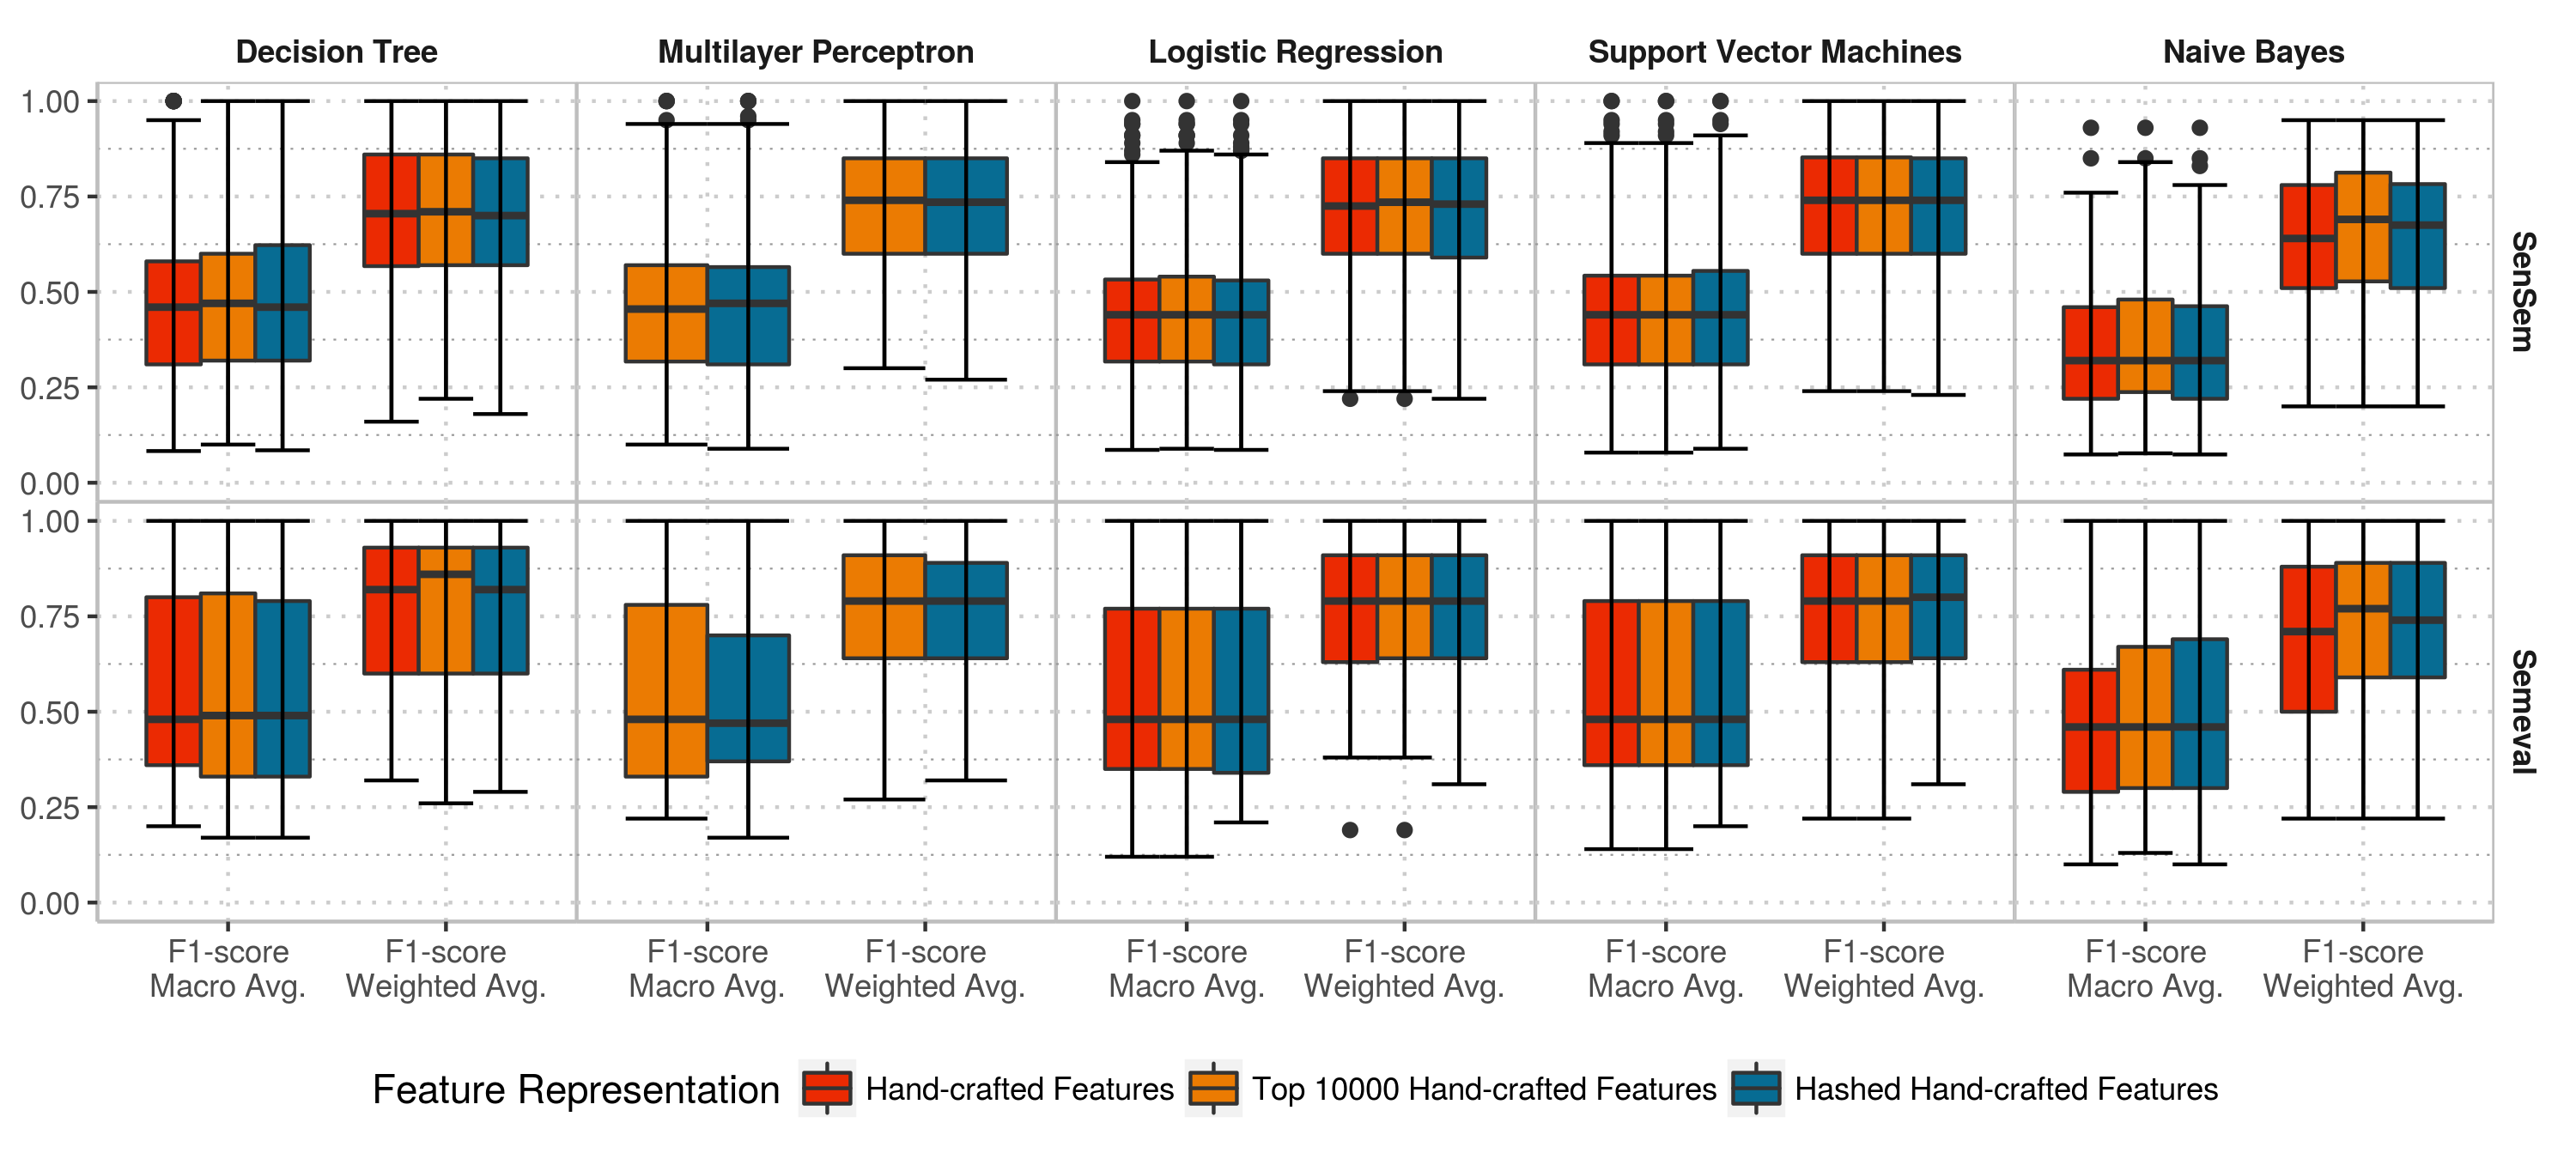
\includegraphics[width=\textwidth]{plots/supervised/representation_comparison}
  \caption{Comparison of feature representations for different classifiers
  using F1-score macro and weighted average}
  \label{fig:supervised:representations}
\end{figure}

Figure \ref{fig:supervised:representations} showcases the different results
of the different models changing the features representation using a box and
whiskers plot. The plot is structured in the following way: 

\begin{itemize}
  \item Each row shows the results for a corpus: SenSem and SemEval.
  \item Each column represents a classifier: decision tree, multilayer
    perceptron (with two hidden layers one of 250 neurons and the other with
    100 neurons), naive Bayes, logistic regression, and support vector
    machines.
  \item Each group of box-plots in each plot represents a metric: F1-score
    macro average and F1-score weighted average.
  \item Each box-plot of different color inside a group is the type of
    representation: all the features, top 10 thousand features selected by the
    feature selection method, and hashed features.
  \item The box and whiskers plots represent the distribution of the values of
    the metrics through their quartiles. Each value is the performance for a
    lemma of the corpus. The black thick line in the middle of a box-plot
    represents the median and the whiskers at the end of each box-plot
    represents maximum and minimum value (except for eventual outliers
    represented by black dots outside the box-plot).
\end{itemize}

First thing to notice in the Figure is the absence of a representation box-plot
in the column corresponding to the multilayer perceptron. This is because of
what was said in the previous paragraph, about a multilayer perceptron being
unable to handle all possible features.

From the graphic I can figure out that there is no distinctive difference from
one representation to the other. In general terms the quartiles are similar,
and the performance depends more on the classifier than the representation. It
is true however that in many (if not all) cases there is a minimal improvement
on the performance by using dimensionality reduction, probably because it makes
the classifiers overfit less when the noise of rare features is removed.
Although it is also true that the use of a feature selection technique has a
little more performance (though still minimal) than the hashing trick, there
was also a trade off because of the computational cost of doing feature
selection for the classification task, which in future experiments using
semi-supervised techniques would become a heavier problem as the number of new
features grows at high pace.

For these reasons, {\em the rest of the experiments were carried out using the
hashing trick representation} as it shows no great drop in performance over the
test set and it is also the cheapest to work with in computational terms.

\subsection{Classifier selection}

In the following chapters I will focus on working with the multilayer
perceptron classifiers. This, again, is to have a point of comparison
particularly in Chapter \ref{chapter:ladder} as Ladder Networks are based on a
multilayer perceptron classifier. It is however important to compare the
multilayer perceptron against other classification methods in order to rule out
the possibility of it being a bad choice to work with from the start.

\subsubsection{Architecture selection}\label{sec:supervised:architecture:selection}

One of the main hyperparameters for a neural network is the architecture.  In a
multilayer perceptron this is the selection of the number of layers and size of
each layer (i.e. number of neurons). As the amount of data is small, there is a
high risk of the network memorizing the datasets. With enough neurons
available, each instance can be mapped to a path in the network.  Thus I cannot
work with a very deep neural network without falling into this problem. That is
why I only look up to three hidden layers.

\begin{figure}[ht]
	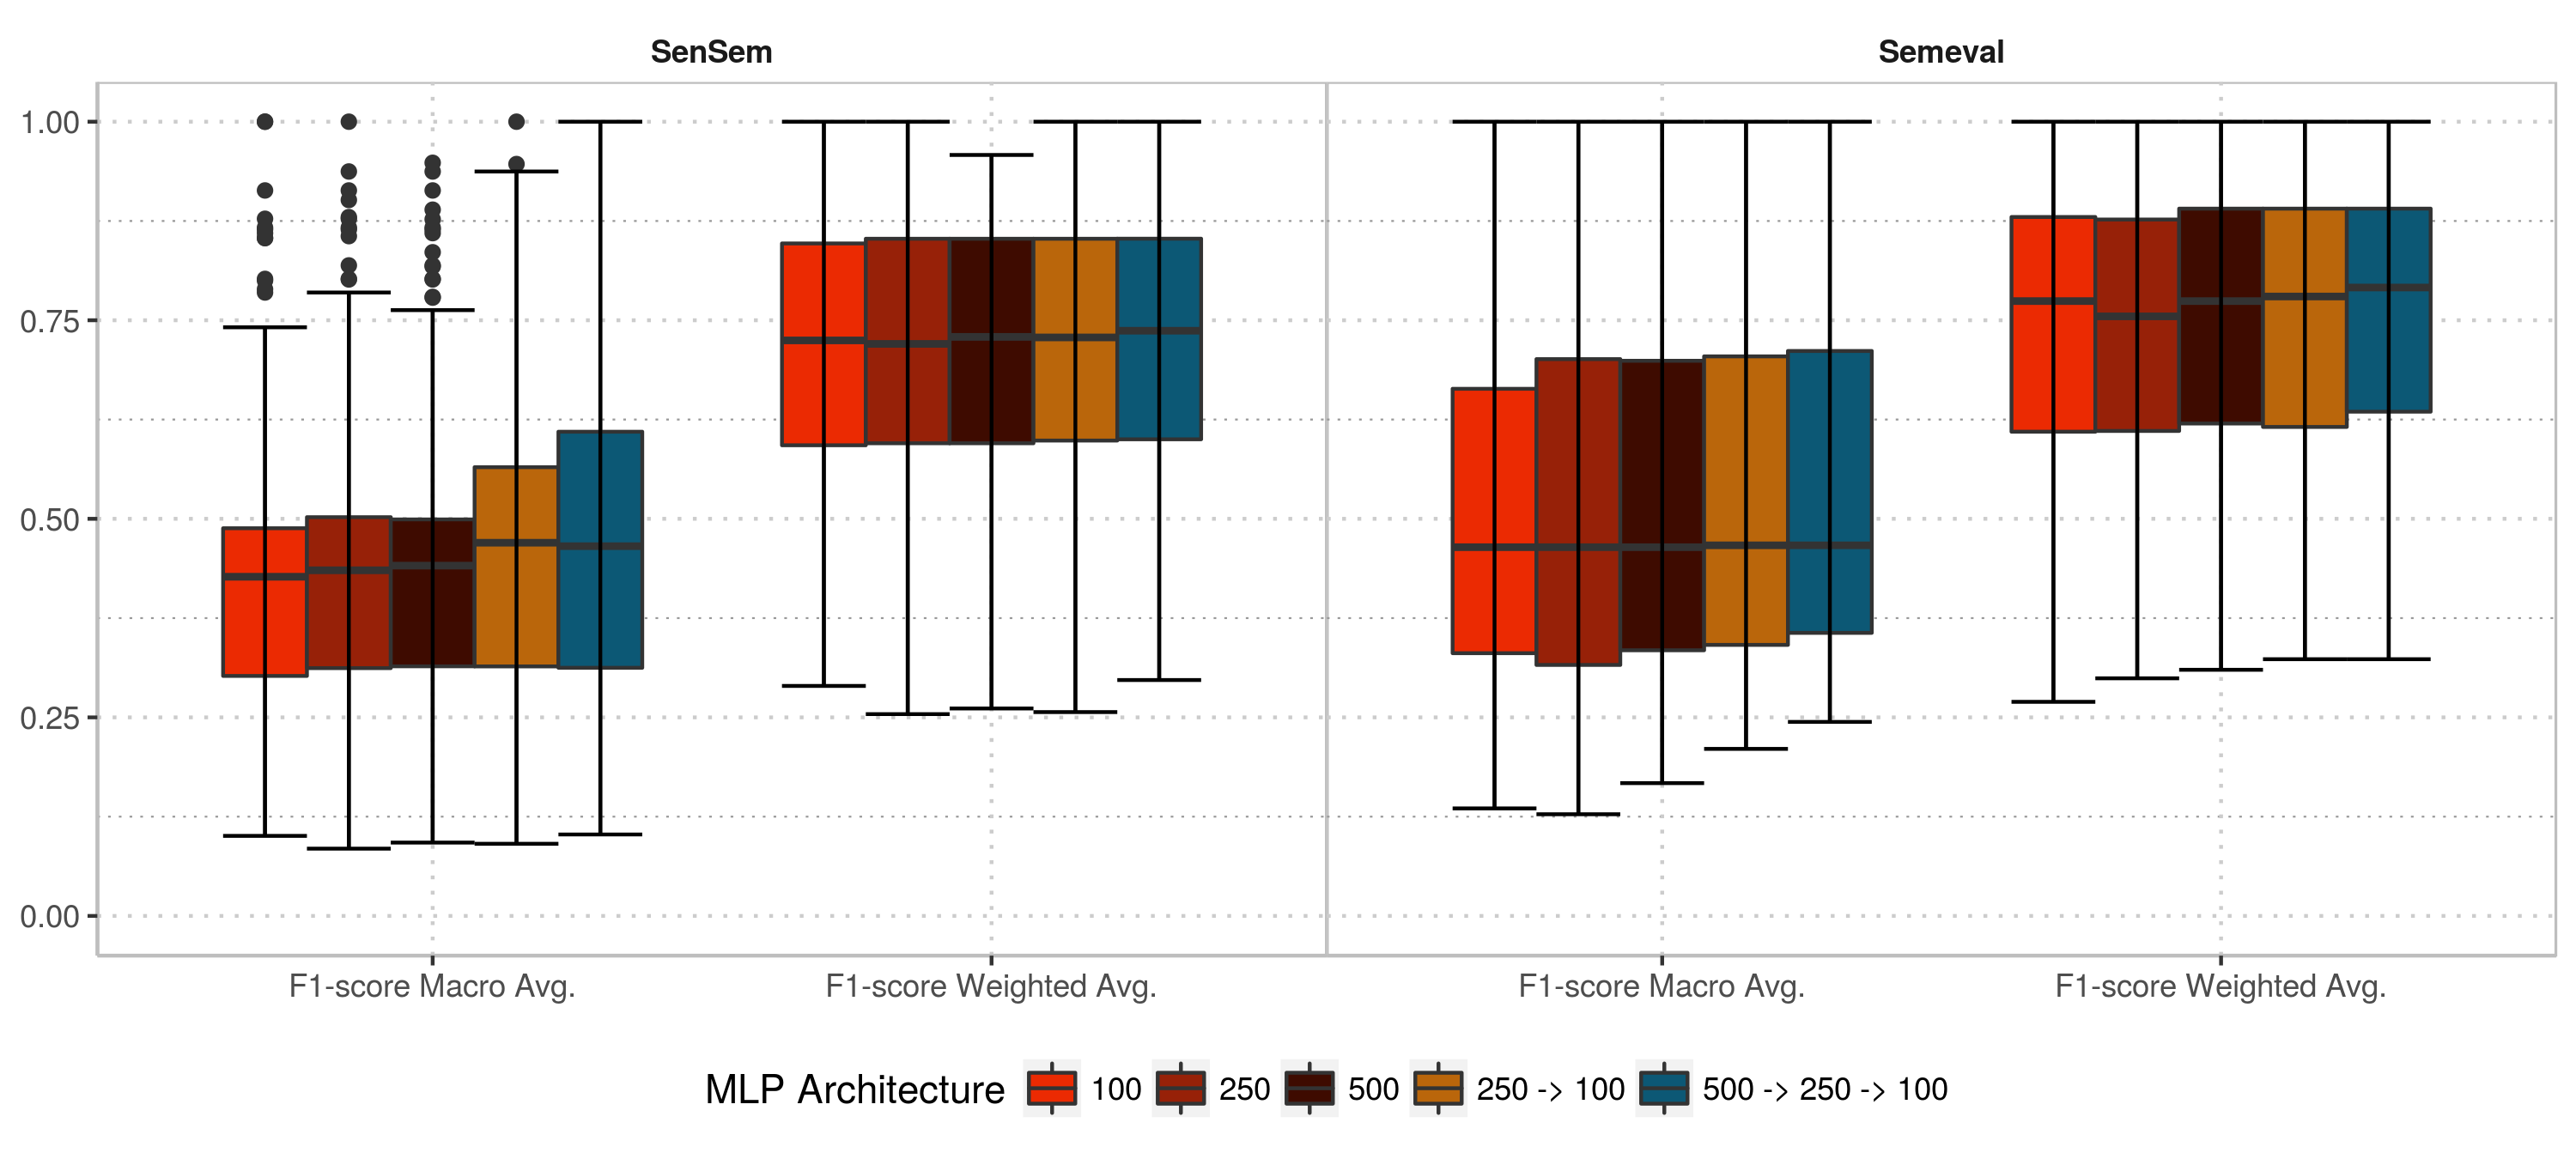
\includegraphics[width=\textwidth]{plots/supervised/mlp_comparison}
  \caption{Comparison of multilayer perceptron architectures}
  \label{fig:supervised:mlp}
\end{figure}

Figure \ref{fig:supervised:mlp} compares different architectures
for a multilayer perceptron using the hashing trick representations (as it was
selected before). This is done only for the following architectures:

\begin{enumerate}
  \item A hidden layer with 100 neurons.
  \item A hidden layer with 250 neurons.
  \item A hidden layer with 500 neurons.
  \item Two hidden layers: the first with 250 neurons, and the second with 100
    neurons.
  \item Three hidden layers: the first with 500 neurons, the second with 250
    neurons, and the third with 100 neurons.
\end{enumerate}

The Figure has a similar structure to that of Figure
\ref{fig:supervised:representations} as it is also a box and whiskers plot
to showcase the performance of each lemma:

\begin{itemize}
  \item Each column represents the corpus: SenSem and SemEval.
  \item The group of box-plots represents the metric: F1-score macro average
    and F1-score weighted average.
  \item Each box-plot of different color represents an architecture of the
    network as described before.
  \item The box and whiskers plots represent the distribution of the
    performance for each lemma as described for Figure
    \ref{fig:supervised:representations}.
\end{itemize}

In this case I can see that the number of neurons does not affect the result
but the number of layers does. The three layer architecture shows the best
results avoiding a high tendency to overfit. There were some other experiments
adding more layers but the improvement on the results was not much more than
with a three layer architecture and, as the number of hyperparameters grow, the
networks were more prone to overfit the data by memorizing it. Plus, the
training time became considerably higher for deeper architectures.

\subsubsection{Comparison of
classifiers}\label{sec:supervised:classifier:comparison}

Figure \ref{fig:supervised:classifiers} showcases the comparison of the
classifiers described in Section \ref{sec:supervised:classifiers}, with an
addition of a baseline classifier which assigns the most frequent sense to every
instance. 

\begin{figure}[ht]
	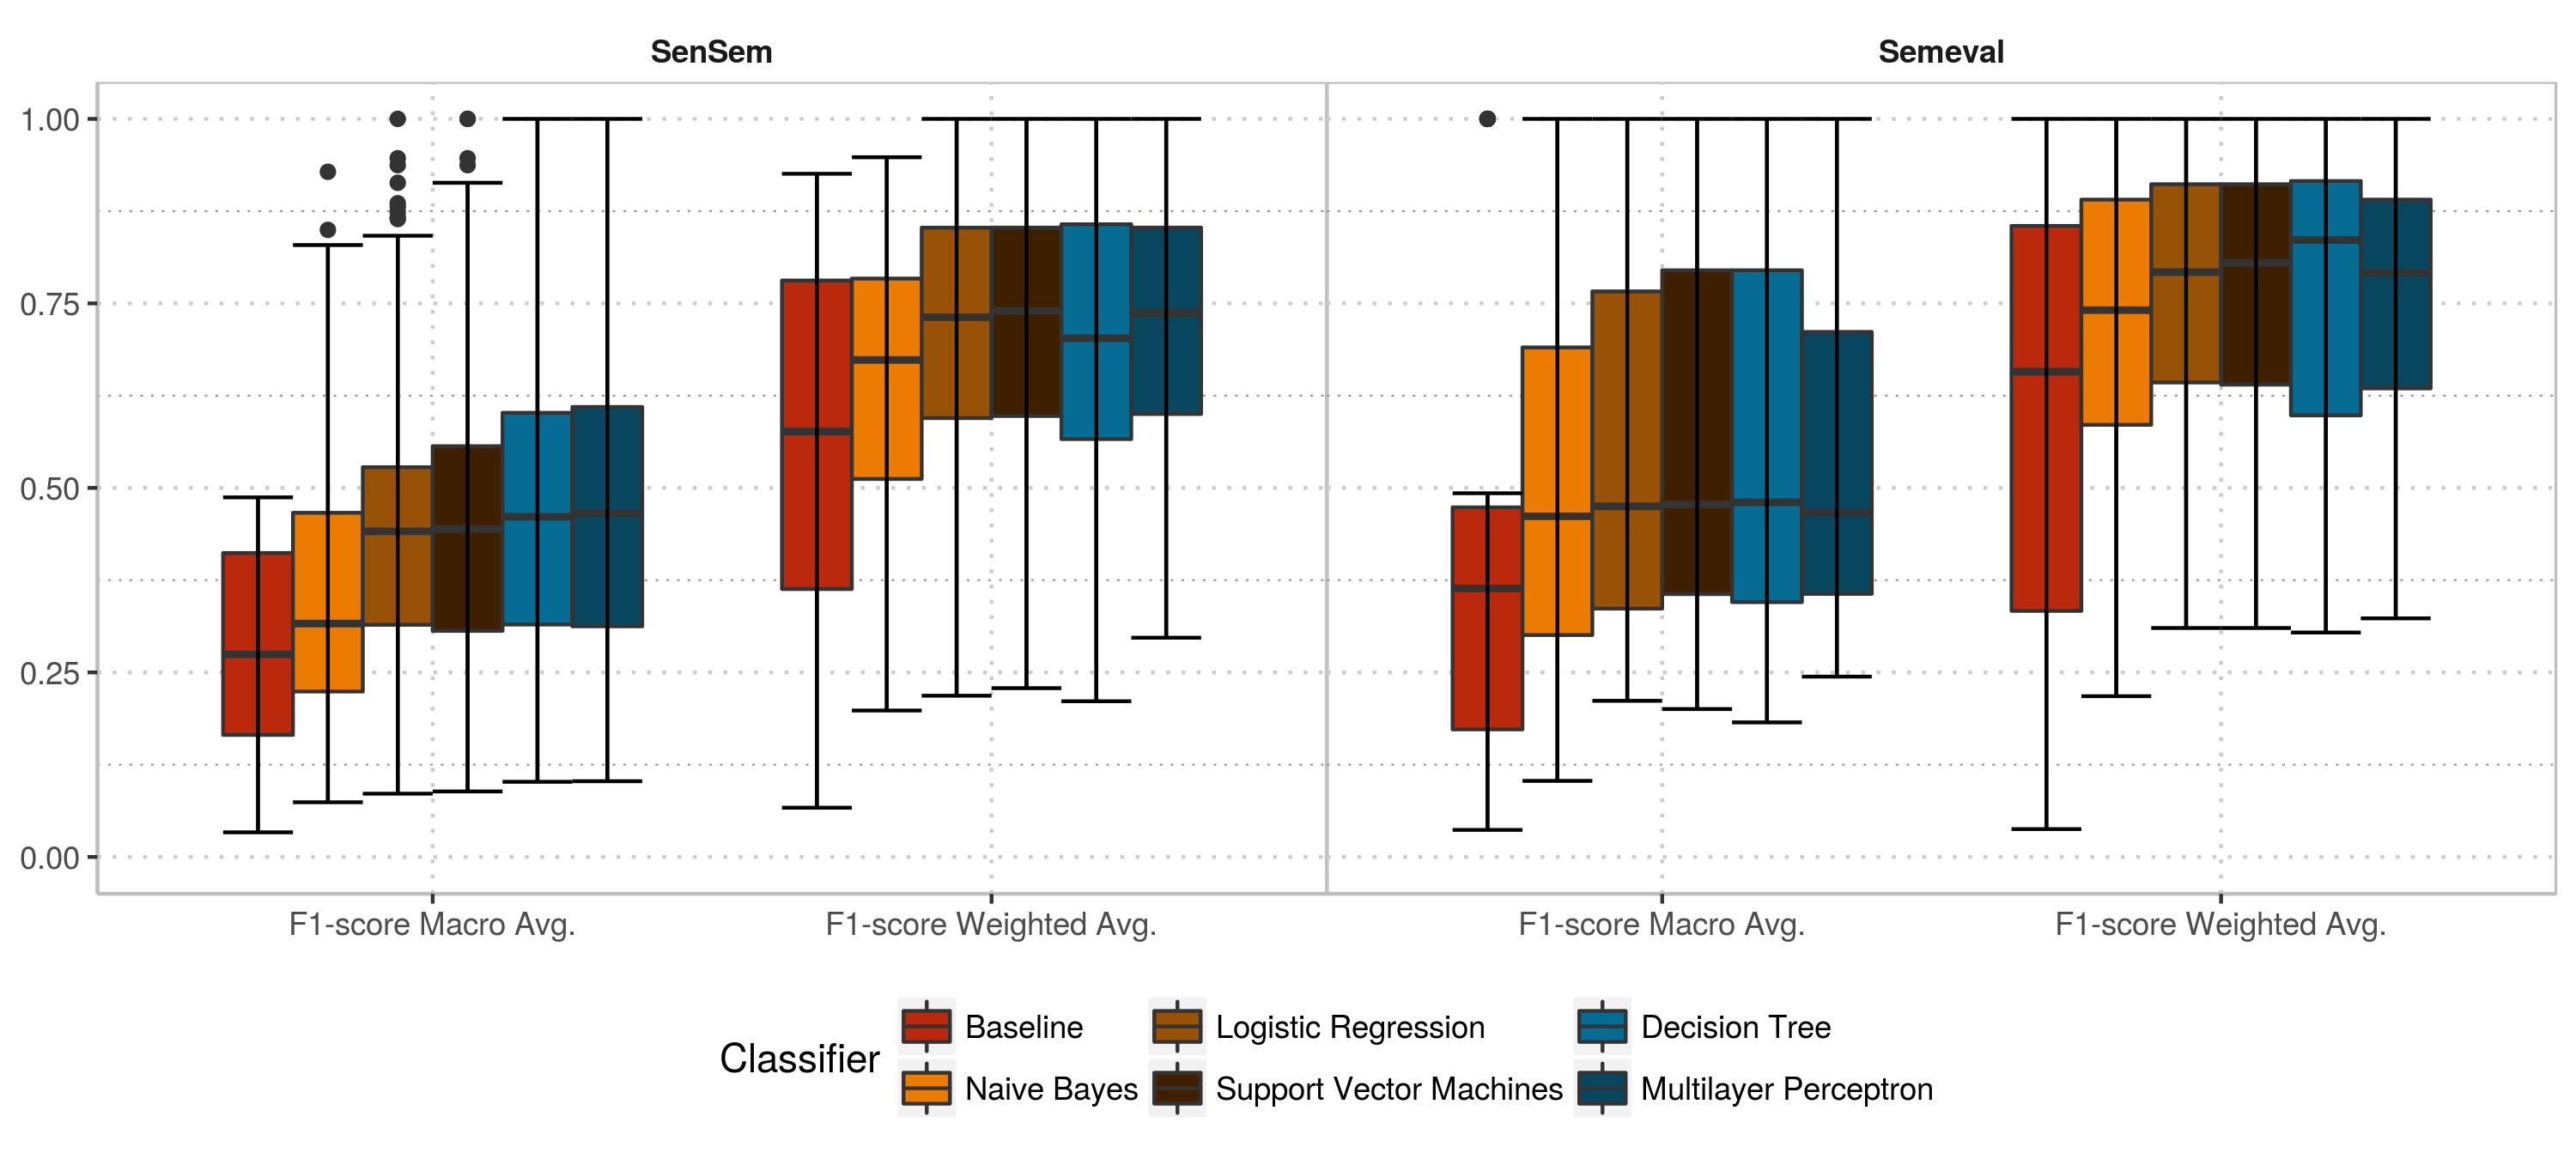
\includegraphics[width=\textwidth]{plots/supervised/classifier_comparison}
  \caption{Comparison of classifiers}
  \label{fig:supervised:classifiers}
\end{figure}

Since it was established that the supervised representation to use in the rest
of the experiments of this thesis is using the hashing trick, the comparison
here is only for such representation. The Figure also has a box and whiskers
plot with a similar structure to that previously shown:

\begin{itemize}
  \item Each column shows the results for a corpus: SenSem and SemEval.
  \item Each group of box-plots represents a metric: F1-score macro average and
    F1-score weighted average.
  \item Each box of different colors inside a group is the classifier:
    baseline, decision tree, multilayer perceptron, naive Bayes, logistic
    regression, and support vector machines.
  \item The box and whiskers plots follows what is described previously
    for Figure \ref{fig:supervised:representations}.
\end{itemize}

First thing to strike out from the plot is that all the classifiers outperform
the baseline classifier described above. In particular, naive Bayes is the one
to show the worst results among the other classifiers, very near to the
performance of the baseline classifier, clearly biased by the most frequent
sense. On the other hand, the decision tree classifier as well as the
multilayer perceptron classifier (with the architecture defined in the previous
section) show the best performances for SenSem corpus if we focus in minority
classes. However, in a weighted average the decision tree has a worse
performance than SVM, LR or MLP.

For SemEval there is less disparity between the performance of the classifiers
(still being naive Bayes the one with worse performance, besides the baseline),
with the median being similar for all of them, and being the decision tree the
one having the best performance in a weighted average. 

Seeing that decision trees and multilayer perceptrons are the ones with the
best performances, there is a strong indication that the problem of
\vsd~is non-linear.

\subsubsection{Significance}

The previous results are good enough to assert that a multilayer perceptron is
a good approach to model the problem of \vsd. However, in order to see whether
the difference in performance is significant or not, I should test it using
Metric \ref{met:2} and seeing the Cohen's kappa coefficient between the
different classifiers.

\begin{figure}[ht]
	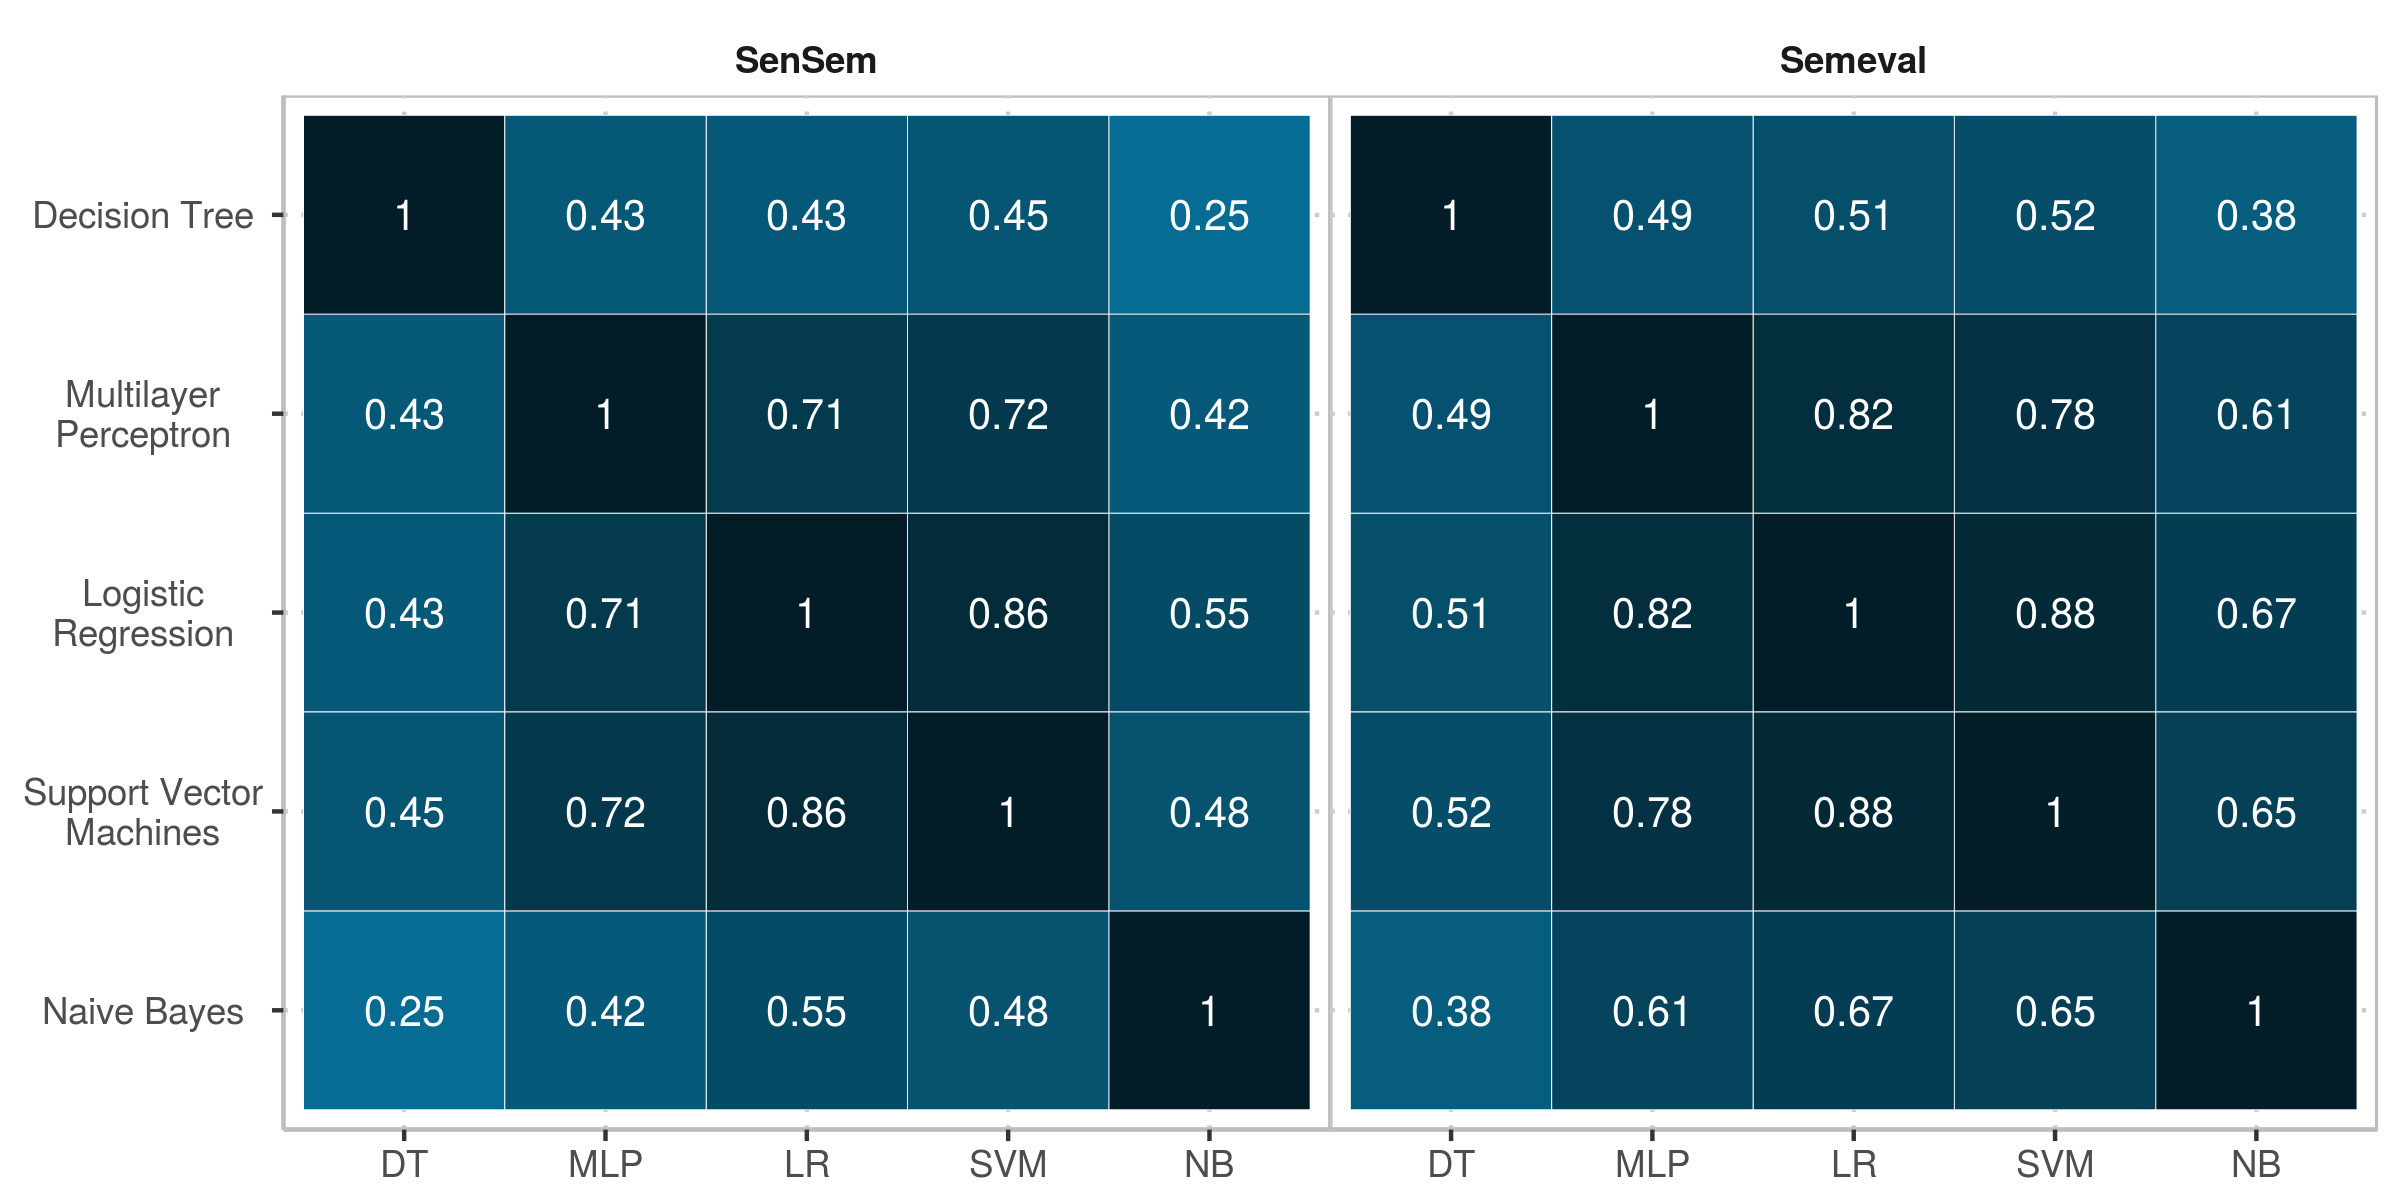
\includegraphics[width=\textwidth]{plots/supervised/inteclassifier_kappa}
  \caption{Cohen's kappa coefficient between classifiers}
  \label{fig:supervised:kappa}
\end{figure}

Figure \ref{fig:supervised:kappa} shows with a heatmap the mean of the Cohen's
kappa coefficient between the classification results of each classifier per
lemma over the test corpus. The higher the kappa, the more similar the
classification, thus the less significant the difference between classifiers.
The color of the heatmap defines the value for inter-classifier kappa between
the classifier of the row and the classifier of the column. The heatmap is
symmetric.

The logistic regression and SVM classifiers are the ones having the most
agreement, probably because they are both linear classifiers. Thus the
difference in performance between them is not really significant. The
multilayer perceptron is the most similar to these two. Decision trees and
naive Bayes are the ones to show the less agreement compared to the other
classifiers. Naive Bayes is likely to have a low agreement as it is one of the
classifiers with worse performance. Although it is not trivial to set a
threshold for which the kappa statistic is good to denote statistical
significance, I can infer from this plot that decision tree learning is clearly
having good performance with statistically significant difference with other
classifiers that are also performing well, which makes it more interesting to
continue exploring in future work. 

\subsection{Hypothesis \ref{hyp:supervised:1}}\label{sec:supervised:hyp:1}

Once the base model to work with for the following experiments is selected, I
can start testing the hypotheses set in Section \ref{sec:supervised:overview}.

I start by looking at the results to test Hypothesis \ref{hyp:supervised:1}.
Recall the hypothesis states that larger training datasets help improving the
performance. To check the validity of this I follow the steps of Experiment
\ref{exp:supervised:2}. I use the multilayer perceptron with three layers
I selected in previous paragraphs.

\begin{figure}[ht]
	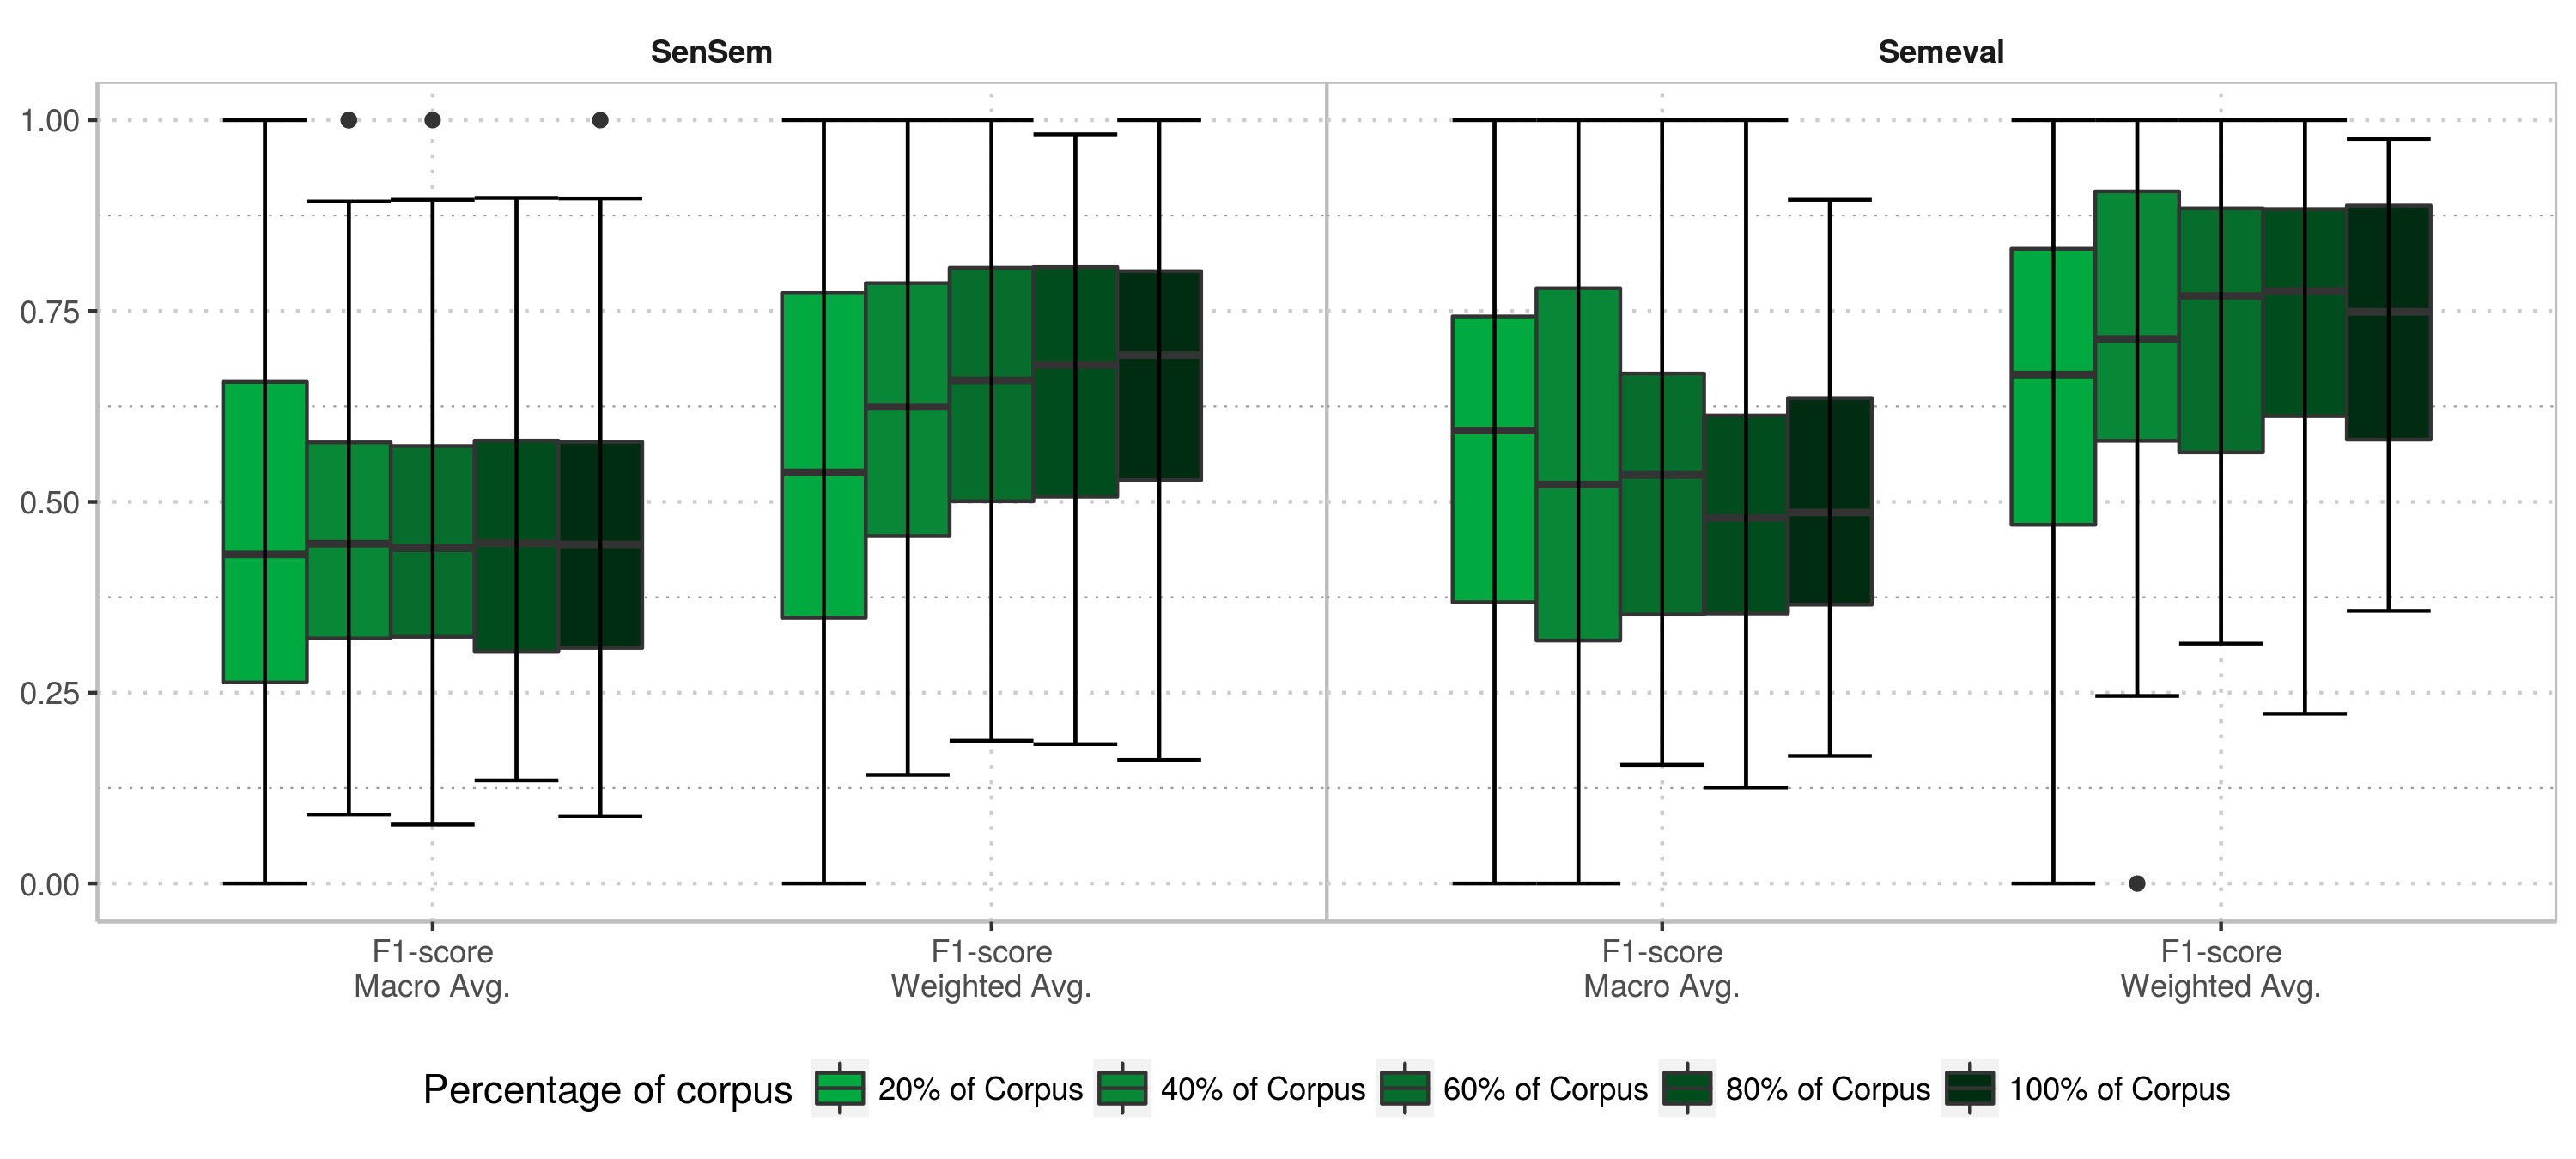
\includegraphics[width=\textwidth]{plots/supervised/performance_progress}
  \caption{Performance per lemma on the test corpus for different sizes of
  training corpus}
  \label{fig:supervised:performance_progression}
\end{figure}

Figure \ref{fig:supervised:performance_progression} shows the performance on
the test corpus for different sizes of the training corpus (as a percentage of
the full training corpus). The figure shows a box and whiskers plot following 
a similar structure shown before:

\begin{itemize}
  \item Each column shows the results for a corpus: SenSem and SemEval.
  \item Each group of box-plots shows the different metrics: F1-score macro
    and weighted average.
  \item Each box-plot of a different shade of color shows the performance for
    different sizes of the training set (as percentage of the total training
    data).
  \item Each box and whiskers plot follows what is described previously for
    Figure \ref{fig:supervised:representations}.
\end{itemize}

The first thing to note from this figure is how, increasing the number of
examples does not necessarily improve the performance of the classifier. This
is due to the fact that in the process to progressively enlarge the corpus
examples are added aiming to have each class represented. When the corpus is
very small, minority classes are comparatively well represented. But as the
number of examples increases, the imbalance between classes also increases.
This results in no performance gain (SenSem) or even degradation of the
performance (SemEval)for minority classes, as can be well seen in the macro
average metric. The weighted average improves with the number of examples in
the case of SenSem, which is a very small corpus, but not so much in the case
of SemEval, which is much bigger. Thus increasing the number of examples seems
good to improve a small corpus but not necessarily a bigger corpus. The main
reason for this seems to be the problem of class imbalance, that becomes more
and more acute as the number
of examples increases.

This however is difficult to see clearly, as the box-plots are useful for
giving a general idea of the performance for many different models, but they
obscure the particular performance of a specific model. As I have one model per
lemma, I would need to examine more closely 200 hundred different models to see
how it is working for each lemma, something outside the scope of this thesis.

There is a clear pattern nevertheless in how a model improves performance with
more training data, specially in cases of models with extremely low
performance: there are models that initially have an F1-score of 0 for the
models trained with the less data, something that does not happen with more
added data.

\subsection{Hypothesis \ref{hyp:supervised:2}}\label{sec:supervised:hyp:2}

To check Hypothesis \ref{hyp:supervised:2} I recall that I would do so
with aid of Experiment \ref{exp:supervised:3}. The hypothesis states
that the size of the dataset not only affects the performance (measured by
Metric \ref{met:1}), but also the tendency to overfit (measured
by Metric \ref{met:3}) of a model.

\begin{figure}[ht]
	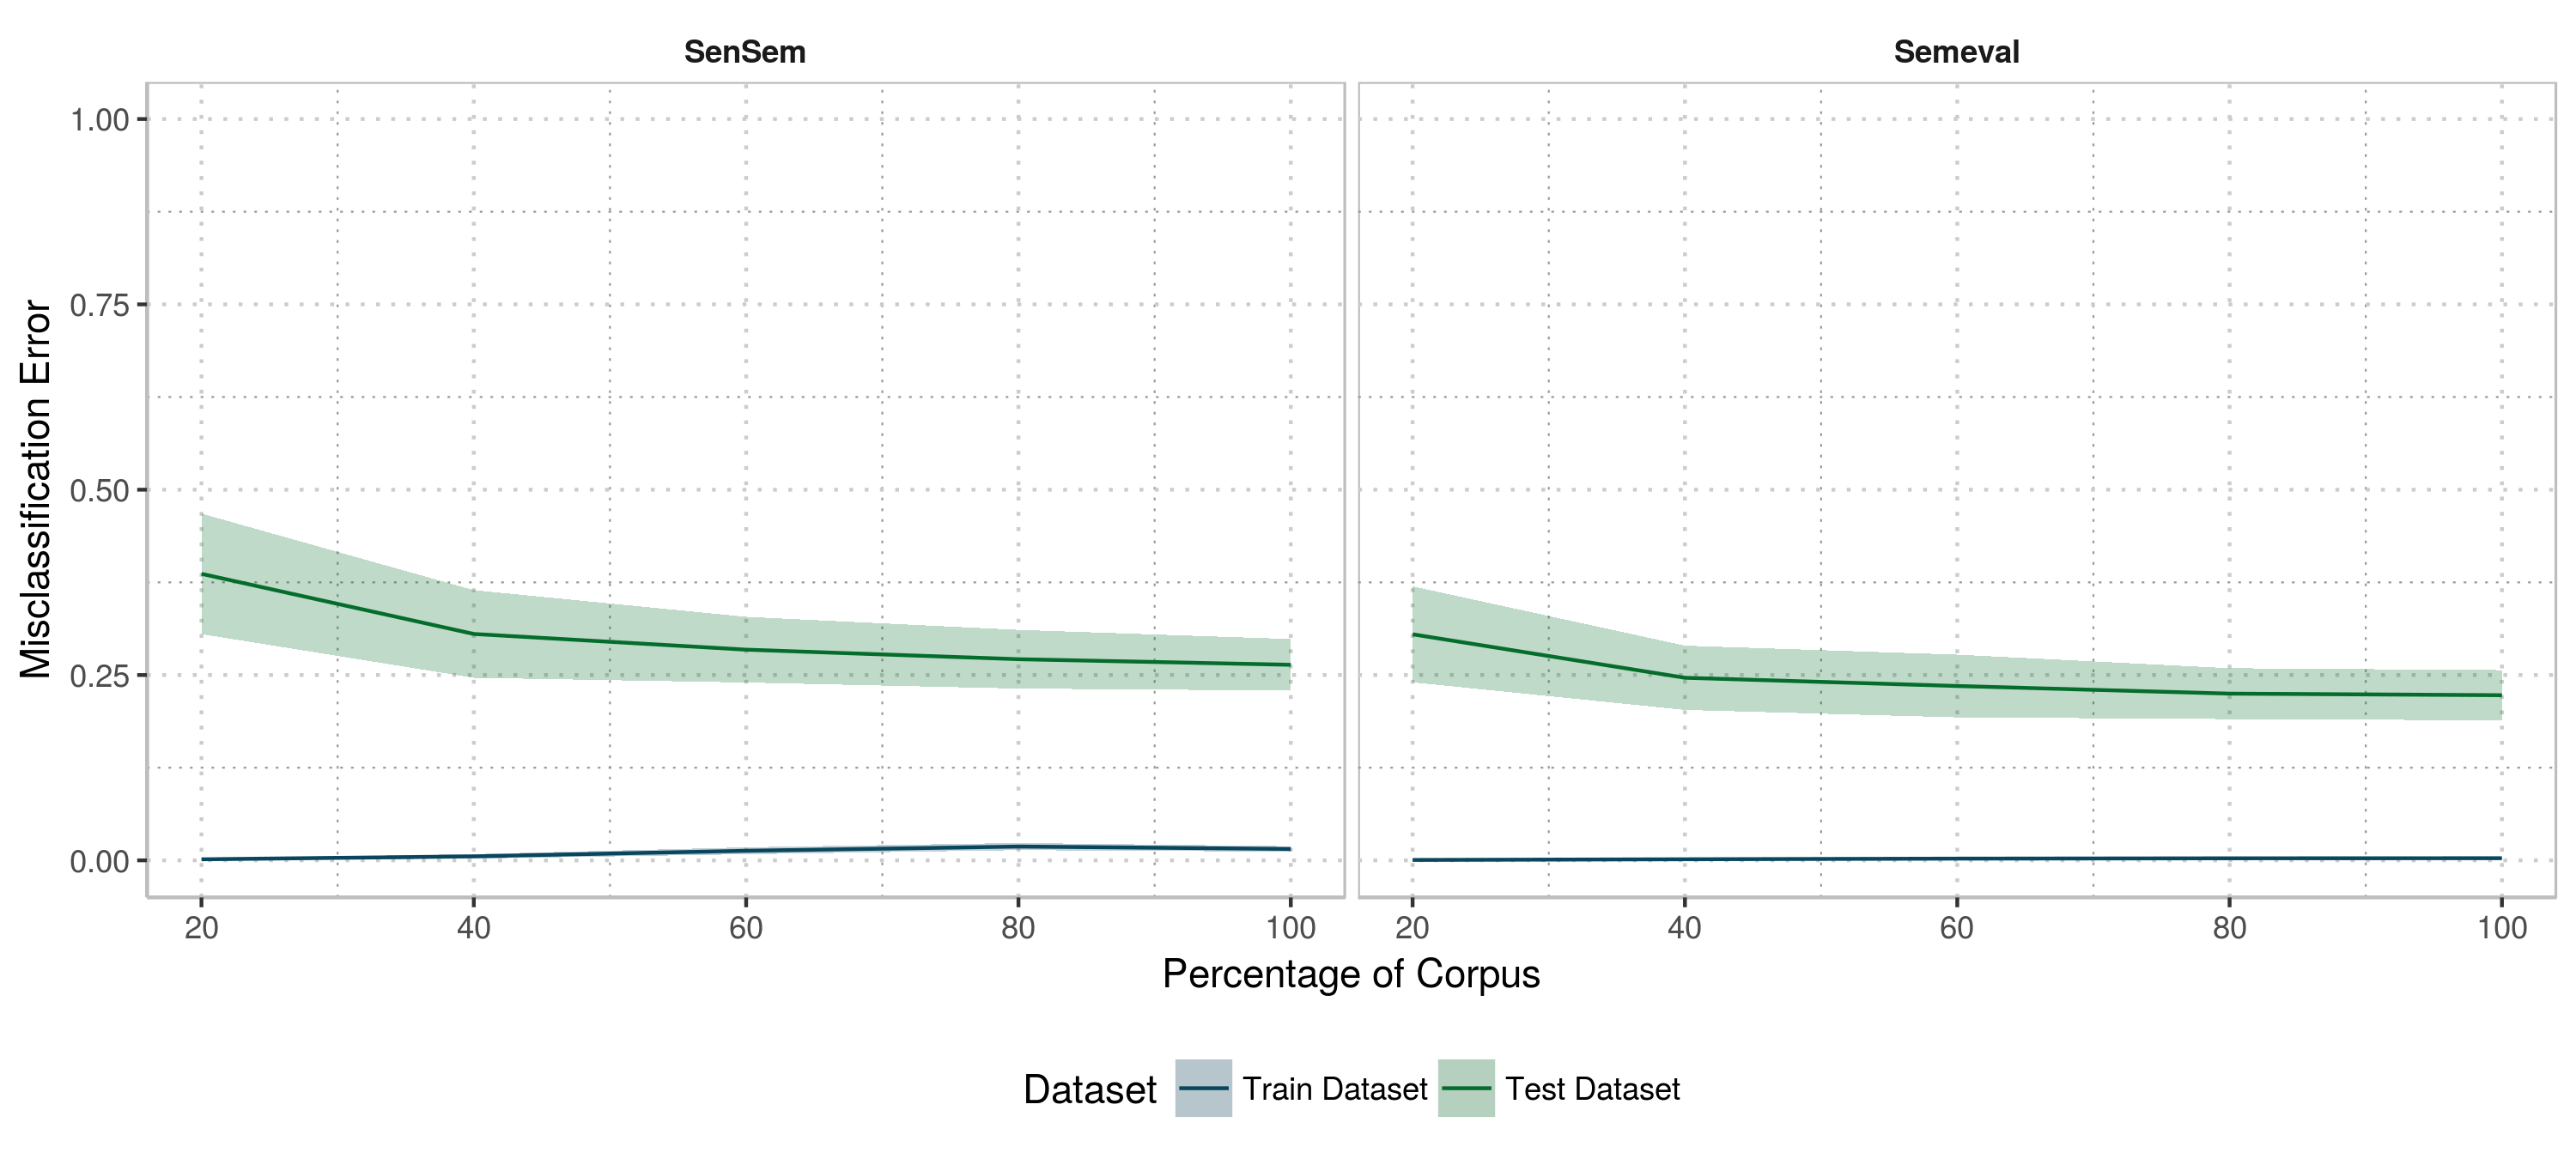
\includegraphics[width=\textwidth]{plots/supervised/learning_curve_scores}
  \caption{Learning curve for different sizes of training corpus}
  \label{fig:supervised:learning_curve}
\end{figure}

Figure \ref{fig:supervised:learning_curve} shows the learning curve for
different sizes of the training data. The structure of the learning curve plot
is as follows:

\begin{itemize}
  \item The plot is divided in two columns, each represents a corpus: SenSem
    and SemEval.
  \item The x-coordinate shows the size of the training data, as a percentage
    of the total training data available, starting from 20\% of the corpus (the
    corpus was split in 5 parts according to Experiment
    \ref{exp:supervised:3}).
  \item The y-coordinate shows the misclassification error of a model.
  \item There are two colors representing the datasets: train and test.
  \item The solid darker lines represent the mean of misclassification error
    trough the different splits of the datasets over all the models.
  \item The shadowed area, which have a lighter color, represent the standard
    error of the mean of the misclassification error.
\end{itemize}

Recall Experiment \ref{exp:supervised:3} first split the corpora in uniform
size parts and gradually added those new parts to the training and evaluation
of the model. It trained a model on a portion and evaluated it on the other,
held-out, portion and recorded the results. It repeated the algorithm a number
of times over different ways of splitting the data to see how the same model
behaves on different datasets. Figure \ref{fig:supervised:learning_curve}
shows the mean and standard error of the mean over the misclassification error
each model has in the training and test datasets.

The test data is having a visible variance of the misclassification error, seen
in the wide shadowed area, while the training data is having almost no
misclassification error, as the shadowed area is indistinguishable of the line
representing the mean of the misclassification error.

In the plot there are two indicators of an error due to variance:

\begin{itemize}
  \item A wider shadowed area: means that the misclassification error of
    different models has a high variance, thus making the models more
    inconsistent over different datasets.
  \item A higher mean of the misclassification error of the test set in
    comparison to the mean training set error, means the model is overfitting
    to the training data.
\end{itemize}

As I clearly see in Figure \ref{fig:supervised:learning_curve}, this variance
is smaller the more training data I have. This is a strong indication of
Hypothesis \ref{hyp:supervised:2} being true, as there is less overfitting in
the different models the more data is used for training.

\subsection{Hypothesis \ref{hyp:supervised:3}}\label{sec:supervised:hyp:3}

To check Hypothesis \ref{hyp:supervised:3} I would do so with aid of
Experiment \ref{exp:supervised:3}. I recall the Hypothesis stated that the
number of classes affects the tendency to overfit (as measured by Metric
\ref{met:3}). To show this I plot the training curve measuring the
mean of lemmas having different number of total labels.

\begin{figure}[ht]
	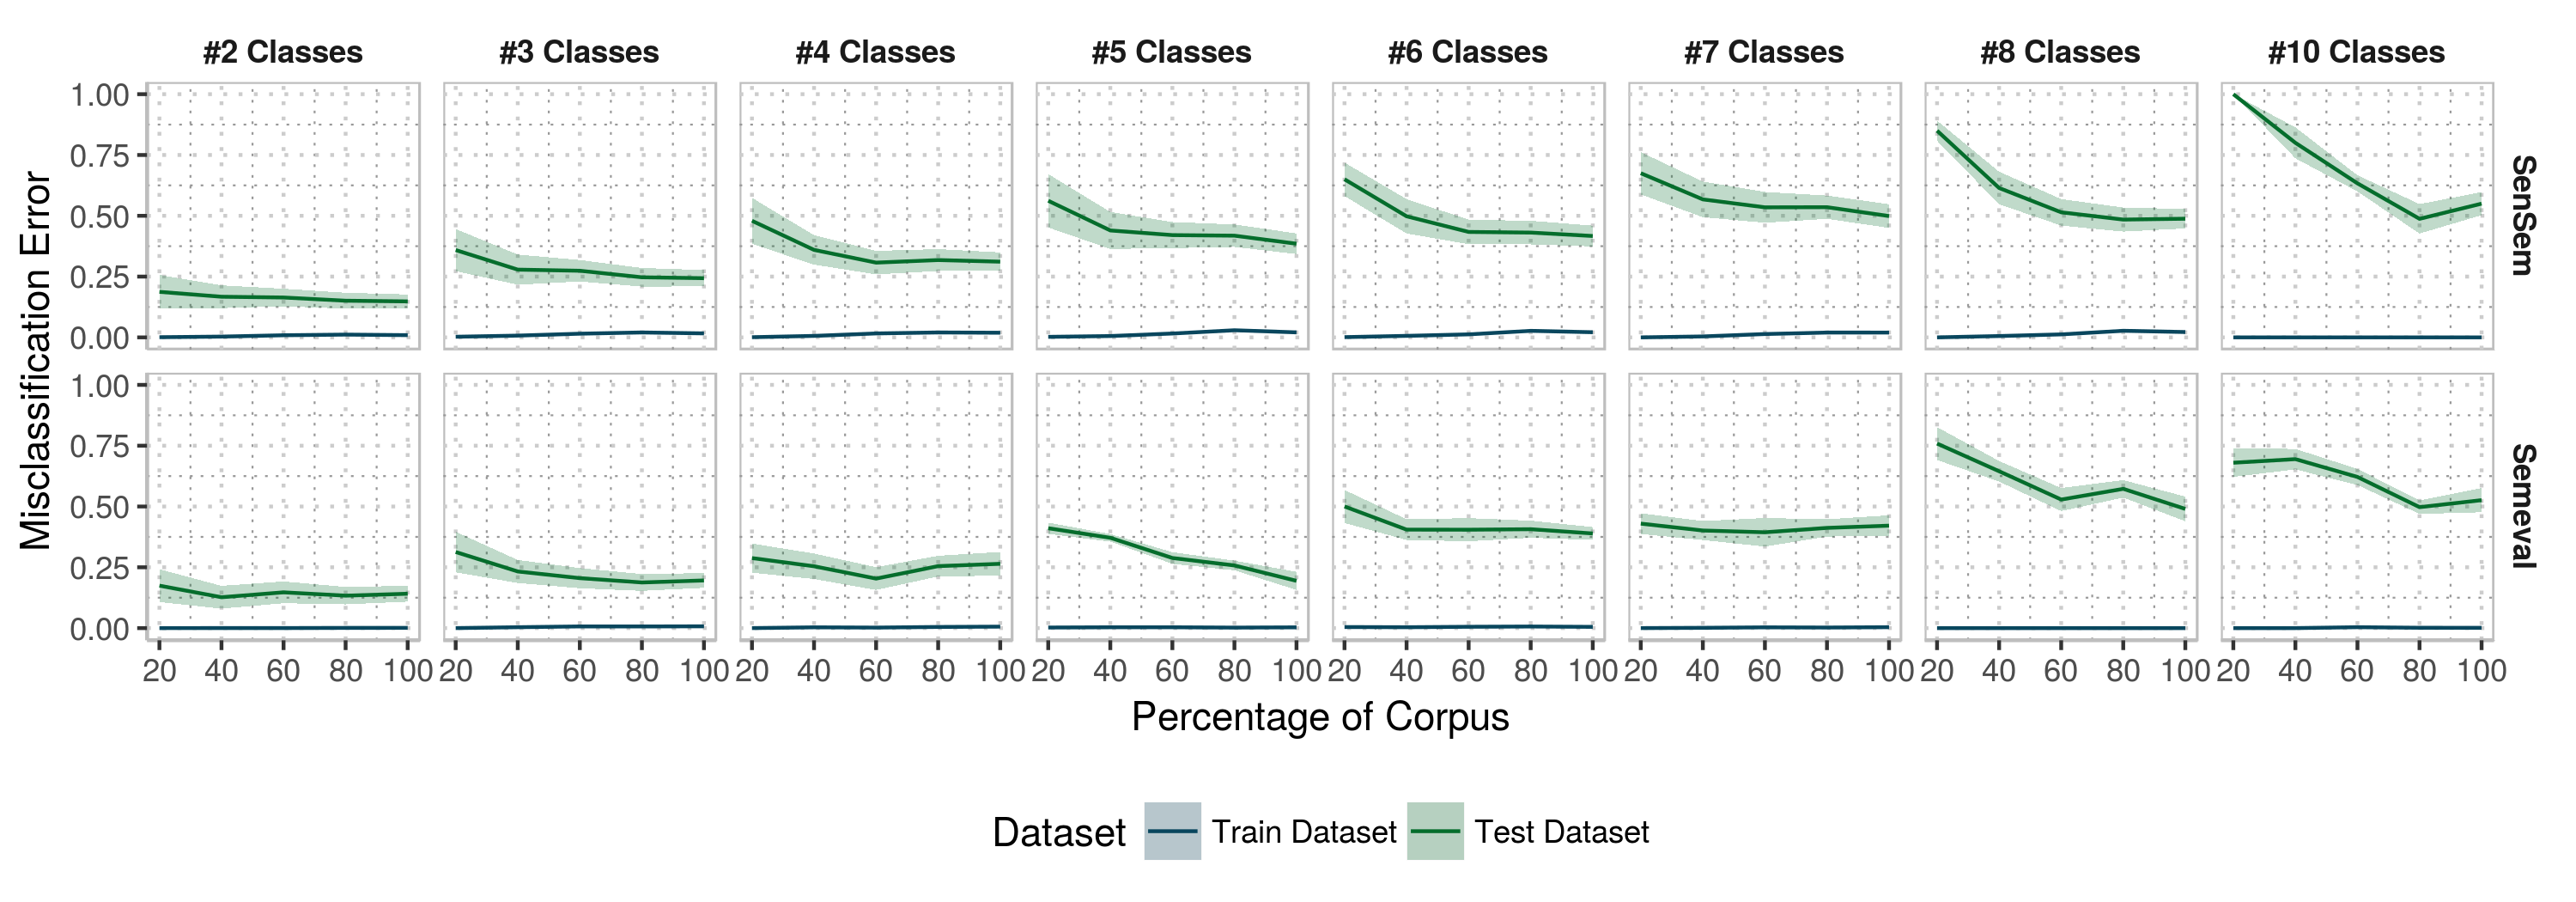
\includegraphics[width=\textwidth]{plots/supervised/learning_curve_per_class_num}
  \caption{Learning curve for different number of classes}
  \label{fig:supervised:learning_curve_per_class_num}
\end{figure}

Figure \ref{fig:supervised:learning_curve_per_class_num} shows the learning
curve for different number of classes. The structure of the plot is similar to
Figure \ref{fig:supervised:learning_curve} with some minor changes to showcase
what the Hypothesis states:

\begin{itemize}
  \item The plot is divided in two rows, each represents a corpus: SenSem and
    SemEval.
  \item The columns of the plots represent the number of classes of the
    models: 2, 3, 4, 5, 6, 7, 8, and 10 classes.
  \item The x-coordinate is the size of the training data as explained in
    Section \ref{sec:supervised:hyp:2}.
  \item The y-coordinate shows the misclassification error.
  \item The colors, lines and shadowed area represent the same thing described
    in Section \ref{sec:supervised:hyp:2}.
\end{itemize}

The models are one for each lemma, thus Figure
\ref{fig:supervised:learning_curve_per_class_num} shows in each column the mean
of all the models having that number of classes (senses). The pattern of the
Figure is clear, as the mean of the error due to variance is larger the more
classes the model has. The error due to high variance is higher in the models
with more classes as a result of the distribution of the classes, which is
Zipfian. As the tendency to classify all the data as part of the most frequent
class when there is not enough data of the other classes, the misclassification
error of the test data is higher than the training error. These results give
evidences to not reject Hypothesis \ref{hyp:supervised:3}.

\subsection{Hypothesis \ref{hyp:supervised:4}}\label{sec:supervised:hyp:4}

To check Hypothesis \ref{hyp:supervised:4} I use Experiment
\ref{exp:supervised:3}. This Hypothesis states that linear models have less
tendency to overfit that non-linear models. This Hypothesis is looking to
check whether the non-linearity of a model affects its tendency to overfit the
data.

\begin{figure}[ht]
	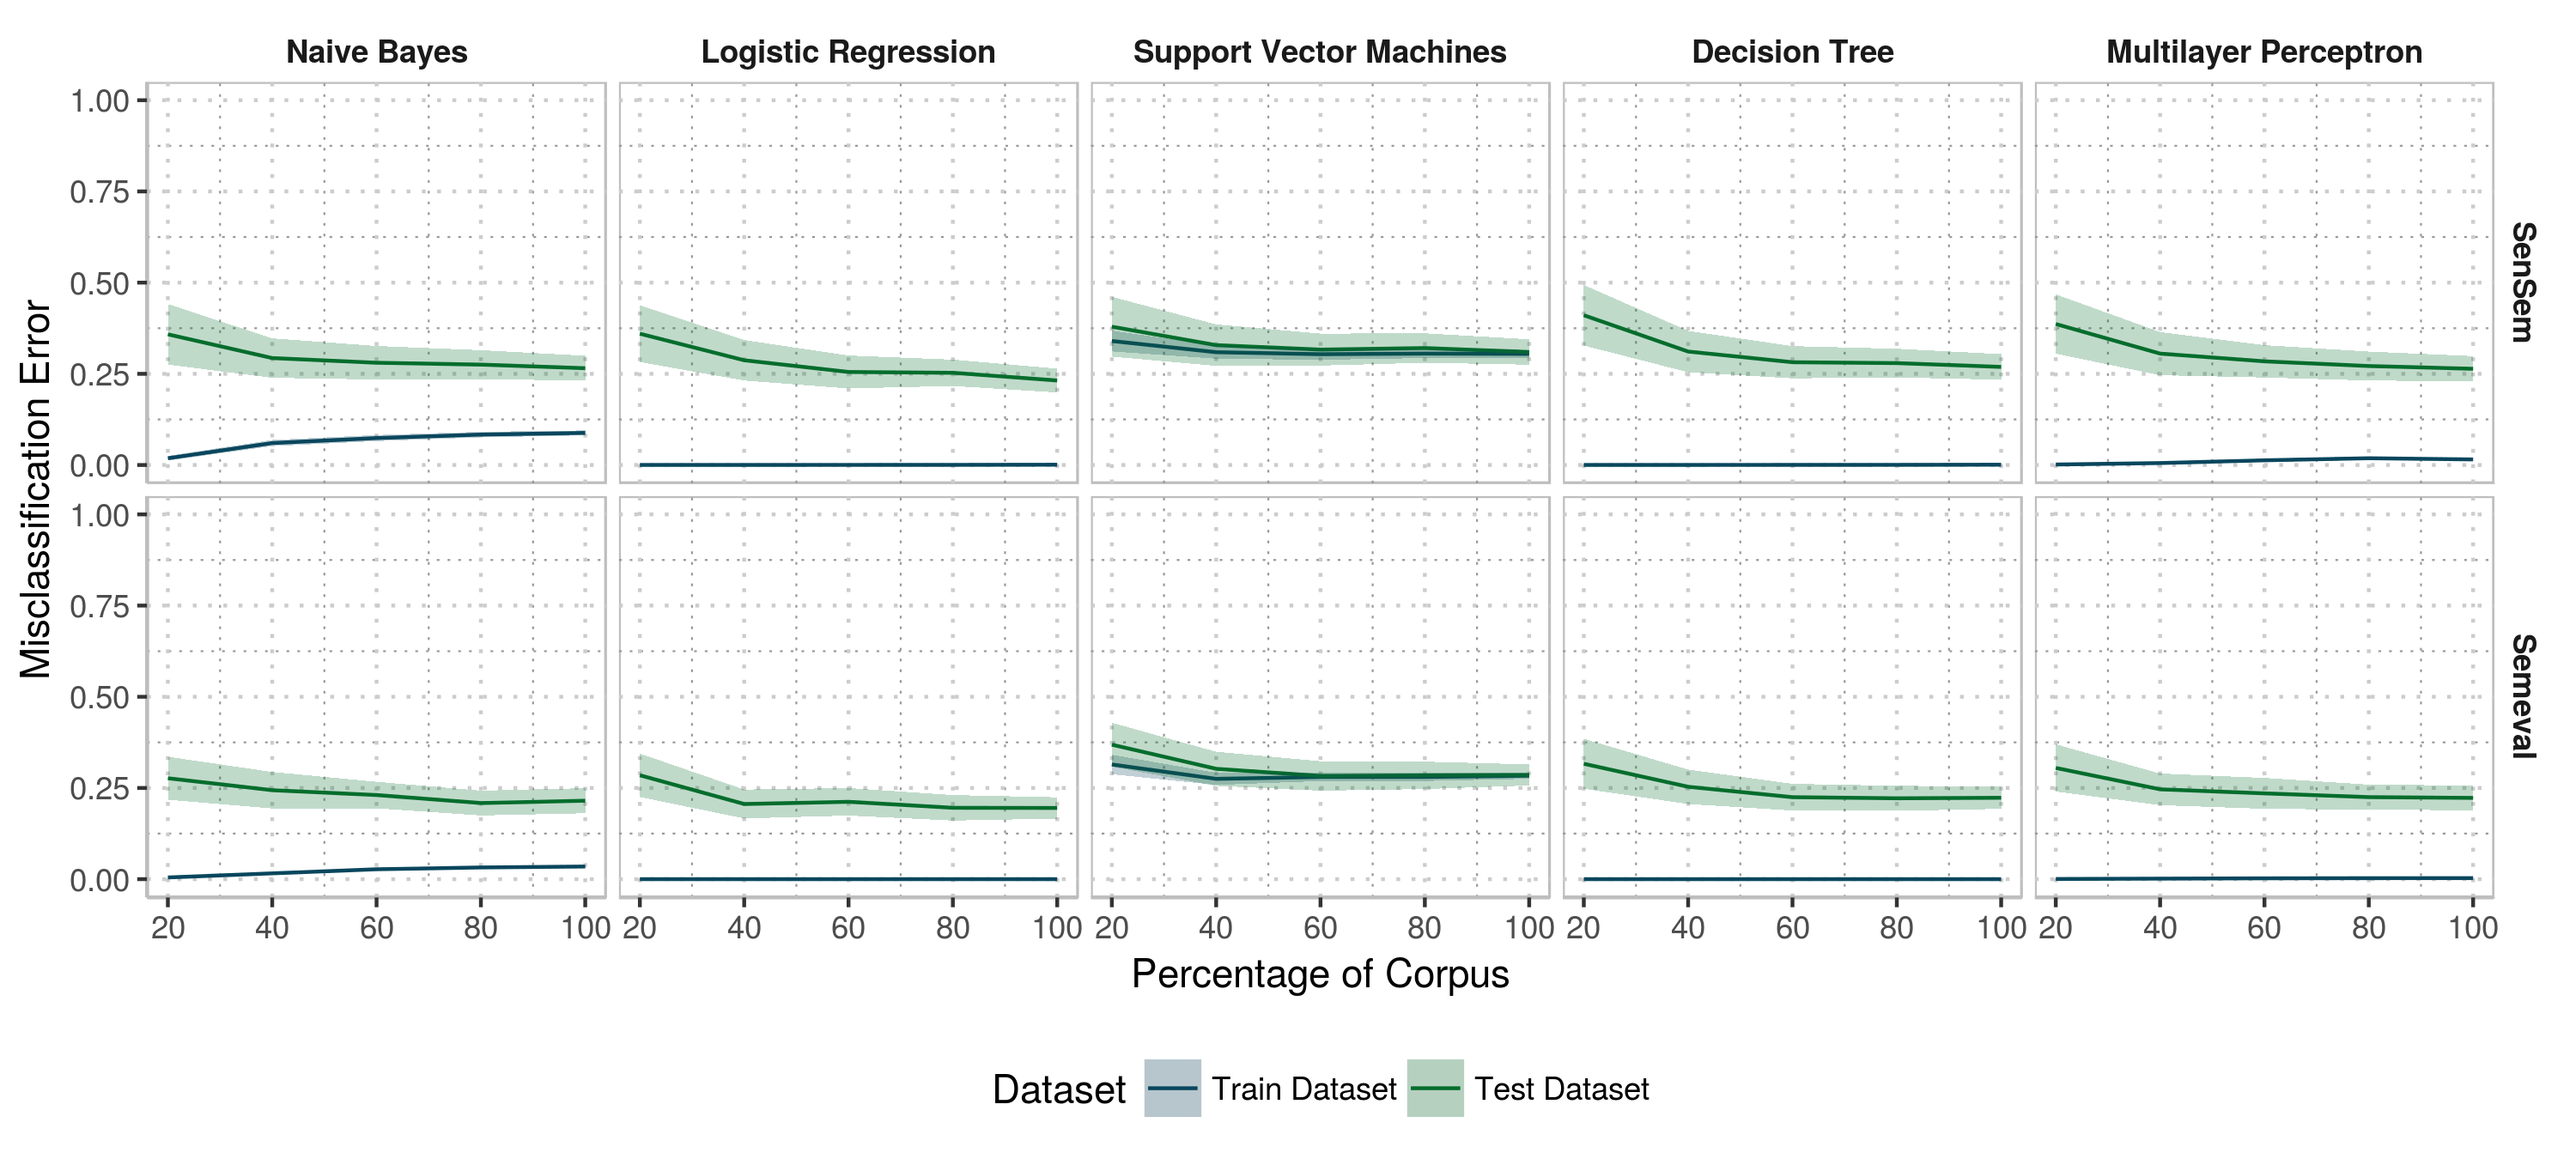
\includegraphics[width=\textwidth]{plots/supervised/learning_curve_per_classifier}
  \caption{Learning curve for different sizes of training corpus per classifier}
  \label{fig:supervised:learning_curve_per_classifier}
\end{figure}

Figure \ref{fig:supervised:learning_curve_per_classifier} showcases the
learning curve for different kind of classifiers (the ones presented in Section
\ref{sec:supervised:classifiers}). The Figure uses a similar structure to that
of Figure \ref{fig:supervised:learning_curve_per_class_num}, but changes what
the columns represent:

\begin{itemize}
  \item The rows of the plot represent the different corpora: SenSem and
    SemEval.
  \item The columns of the plot represent the different classifiers: Naive
    Bayes, Logistic Regression, Support Vector Machines, Decision Tree and
    Multilayer Perceptron. Note that the linear classifiers are the first
    three ones from the left and the non-linear classifier are the last two
    from the left.
  \item The x-coordinate represents the size of the training data as a
    percentage of the total training data.
  \item The colors, lines and shadowed area represent the same thing described
    in Section \ref{sec:supervised:hyp:2}.
\end{itemize}

The first thing that highlight in the plot are the results for Naive Bayes and
Support Vector Machines. In both cases, the training error is not so close to 0
as it is for the other classifiers. 

In Naive Bayes, the error of the training data increases with the number of
training instances. Remember in Section
\ref{sec:supervised:classifier:comparison}, I saw Naive Bayes was the
classifier with the lowest performance and I figure out this was a result of it
being biases towards the most frequent class. Figure
\ref{fig:supervised:learning_curve_per_classifier} gives even more evidence to
support that claim. Naive Bayes then shows less difference between the training
error and the test error as it sacrifices the performance of the model for more
generality of it.

Support Vector Machines shows a wider shadowed area of the training dataset
misclassification error, which means a higher variance of the performance in
the training data. SVM with a linear kernel separates the data with an
hyperplane of maximum margins, just as naive Bayes, it sacrifices good
performance of the training data for a better performance over the general
data.

The other three methods show very similar results, with decision trees being
slightly higher than the rest and logistic regression being slightly lower.
However, from the visual results I see the significance of this difference
in performance is not significant.

The results shown are supportive of Hypothesis \ref{hyp:supervised:4}, as
the linear classifiers show less tendency to overfit, although is at expense
of a higher error due to bias.

\section{Conclusions}\label{sec:supervised:conclusions}

This chapter introduces the problem of \vsd~using purely supervised methods.
The hypothesis I want to test is that the size of the training
set affects the performance of a model. This initial hypothesis was divided
into more specific subhypotheses, which the experimentation and analysis of
results tried to accept or reject.

I designed some experiments to see if there was a significant difference
between different models. A first step was to rule out that techniques to
reduce dimensionality of the representations affected the performance of the
models. This was shown true with the results in Section
\ref{sec:supervised:representation:selection}.

For the neural network classifier, I needed to set the architecture of the
network. The results reported that an architecture with more layers improved
the performance of the model. This was not the case for the number
of neurons per layer. Section \ref{sec:supervised:architecture:selection} shows
these results.

Finally, I compared the performance of the neural network classifier with the
other classifiers defined in Section \ref{sec:supervised:classifiers}. Section
\ref{sec:supervised:classifier:comparison} shows the neural network had one of
the best performances for the SenSem corpus. Nevertheless, the Kappa
coefficient did not report significance in this improvement over the other
classifiers. In any case the objective was to check whether the neural network
was outperformed by other classifiers, which was not the case. The neural
network, as I will show, is the classifier that I finally chose because its
performance was not worse than the others and it is comparable to the
classifiers explored in future chapters.

The experiments done to accept or reject Hypothesis \ref{hyp:supervised:1} that
larger training dataset improve on the performance are observable in Section
\ref{sec:supervised:hyp:1}. The reported results give strong indications about
the validity of the Hypothesis, since there is a visible improvement in the
overall results as the number of training examples increases, thus the
Hypothesis cannot be rejected.

Hypothesis \ref{hyp:supervised:2} cannot be rejected since results of Section
\ref{sec:supervised:hyp:2} give a strong evidence to support it. Indeed,
the tendency to overfit and the error due to variance decrease the more
training data the model has.

In the same way Hypothesis \ref{hyp:supervised:3} cannot be rejected because of
the evidence in results of Section \ref{sec:supervised:hyp:3}. The number of
classes (senses) affects the overfitting of the model. The more classes, the
more difficult for the model not to overfit.

Finally, experiments to test Hypothesis \ref{hyp:supervised:4}, which expects
linear models to have less tendency to overfit than non-linear models, do not
yield conclusive results, although in a shallow observation the results can be
interpreted in favor of not rejecting the Hypothesis. Two of the linear
classifiers have the training error closer to the validation error. The methods
sacrifice accuracy in their training data in order to improve the
generalization. The problem however is that the test set misclassification
error does not look significantly better than for the other classifiers.

The objective for this chapter was to lay the foundations on which the
following chapters will compare and try to overcome its shortcomings. In
particular, the purely supervised models present challenges in two main
aspects: the tendency to overfit when training a model with a small dataset and
the coverage that these models may have over new unseen examples. The
semi-supervised approaches I will explore in the following chapters try to
resolve these challenges from different angles.

One of the latent causes to overfit in purely supervised models is given by the
very nature of such models. They generate a representation of the training
examples based on features obtained from the same annotated data the
classifiers is attempting to represent. The way I aim to attack this flaw is
by using features which generalize better, not tied to a particular labeled
dataset but obtained from a more general language sample. This is explored in
Chapter \ref{chapter:embeddings}. Smoother representations of the labeled
data are used by unsupervised methods with word embeddings.

Another of the latent problems in purely supervised models occur in the
coverage of such models. This is difficult to measure and quantify, since to do
so a much larger number of annotated examples are needed.

The coverage problem can only be measured through the silence metric. Silence
captures those examples that belong to one of the data classes, but are not
available in the annotated corpus, thus models cannot learn from these data.
The annotated data can only consider a limited universe of features, leaving
out other characteristics of the labels that may improve the model on new
candidates to classify.

Other semi-supervised methods, studied in more detail in later chapters, study
ways to overcome this shortcoming of purely supervised approaches, for example, by
annotating new data (automatically or manually) contributing to supervised models
to have more latent information so as to improve the performance over new data.
